With the methods and approaches developed in \autoref{chap:oneD} for the one-dimensional model, we have an expectation of the behavior of the two-dimensional Stommel model around the non-smooth bifurcation under similar conditions. With the bifurcation structure we explored in \autoref{chap:background}, we consider a generalization with the canonical model

\begin{equation}\label{eq:twoD_canonical}
  \begin{aligned}
   \dot{V} & =  \eta_1-\eta_2+\eta_3(T-V)-T-V|V|+A\sin(\Omega t), \\
   \dot{T}     & =  \eta_1-T(1+|V|)+B\sin(\Omega t),  \\
  \dot{\eta_2}  & =  -\epsilon\\
  T(0)&=T_i,\quad V(0)=V_i,\quad \eta_2(0)={\eta_2}_i>\eta_1\eta_3,
  \end{aligned}
\end{equation}

with slow variation $\epsilon\ll 1$, high frequency $\Omega\gg 1$, amplitudes of oscillation $A$ and $B$, and model parameters $\eta_1$ and $\eta_3$ to be fixed positive constants. This is the generalized two-dimensional Stommel model with two additional features. First, we allow for slow variation in the bifurcation parameter, this has been shown to be realistic as the $\eta_2$ is related to the freshwater flux and therefore not a fixed parameter; the same assumption is made in Roberts \cite{roberts2017relaxation}. Second, we consider periodic forcing in the additive parameters ($\eta_1,\eta_2$) to account for oscillations in the observed behavior in Huybers \cite{huybers2005obliquity}. To fully understand the effects of each component on the model, we build them individually before putting them together.

For the remainder of this paper, we make two assumptions: first that $\eta_3<1$ which causes \eqref{eq:twoD_canonical} to admit the smooth bifurcation in the positive $V$ region. The value $\eta_3$ describes the relative strength of the temperature relaxation to that of salinity, and it is frequently assumed that salinity's is much longer, giving $\eta_3<1$. Although not necessary, this will align our focus and give a case to analyze in depth, the case of $\eta_3>1$ follows similarly. The second assumption we make is that even though we have a two-dimensional model, the variable $V$ is leading the dynamics of the system with it's nonlinear behavior. This assumption makes it clear that we will want to understand the non-smooth behavior in $V$ where $T$ follows in response to the effects of $V$. Again, also not necessary as the opposite situation may be considered, there is evidence to show that changes in temperature respond to changes in salinity and this assumption allows for better physical agreement. With this we have the ability to solve behavior of $T$ in terms of $V$ to find equations in only one variable.

\section{Slowly Varying Parameter}
\label{sec:twoD_slow}

We consider only the slow variation mechanism to understand it's effects on the canonical system \eqref{eq:twoD_canonical} with $\epsilon>0$ and $A=B=0$, where we allow the bifurcating parameter to slowly vary but no oscillatory forcing. With the parameter $\eta_2$ slowly varying, we expect to find a tipping point in the neighborhood of the aforementioned non-smooth bifurcation. With the choice of $\eta_3<1$, the lower branch with $V<0$ is the branch we focus on in order to approach the non-smooth behavior, thus \eqref{eq:twoD_canonical} becomes

\begin{equation}\label{eq:twoD_slow_negative}
 \begin{aligned}
   \dot{V} & =  \eta_1-\eta_2(t)+\eta_3(T-V)-T+V^2, \\
   \dot{T} & =  \eta_1-T(1-V),  \\
  \dot{\eta_2}  & =  -\epsilon.
  \end{aligned}
\end{equation}

From \autoref{sec:oneD_slow}, we learned that the one-dimensional model had a solution that began to act differently on a smaller scale. It was this approach that gave insight into the tipping. Here we search for an outer solution to \eqref{eq:twoD_slow_negative} that helps us understand the behavior of system.  Since we have slow variation in the parameter, we choose to scale the system \eqref{eq:twoD_slow_negative} with the 'slow' time $\tau=\epsilon t$

\begin{equation}\label{eq:twoD_slow_slowsystem}
\begin{aligned}
\epsilon V_\tau =&\eta_1-\eta_2(\tau)+\eta_3(T-V)-T+V^2, \\
\epsilon T_\tau & =  \eta_1-T(1-V),  \\
  {\eta_2}_\tau  & =  -1.
\end{aligned}
\end{equation}

We also form an asymptotic expansions in terms of the small quantity $\epsilon$ to get an expression that separates the dynamics by their contribution to the solution. Here we choose

\begin{equation}\label{eq:twoD_slow_outerexpansion}
\begin{aligned}
V(\tau)\sim &V_0(\tau)+\epsilon V_1(\tau)+\epsilon^2 V_2+\ldots\\
T(\tau)\sim & T_0(\tau)+\epsilon T_1(\tau)+\epsilon^2 T_2(\tau)+\ldots
\end{aligned}
\end{equation}

and substitute \eqref{eq:twoD_slow_outerexpansion} into \eqref{eq:twoD_slow_slowsystem} to find

\begin{equation*}
\begin{aligned}
 \epsilon{V_0}_\tau+\epsilon^2{V_1}_\tau+\ldots =&\begin{aligned}[t]
\eta_1-&\eta_2(\tau)+\eta_3(T_0-V_0)-T_0+V_0^2\\
&+\epsilon(\eta_3(T_1-V_1)-T_1-2V_1V_0)+\ldots
\end{aligned}\\
\epsilon{T_0}_\tau+\epsilon^2{T_1}_\tau+\ldots=&\eta_1-T_0(1-V_0)+\epsilon(-T_1(1-V_0)+V_1T_0)+\ldots
\end{aligned}
\end{equation*}

Which once we separate at each order of $\epsilon$ we find the equations

\begin{align}
\label{eq:twoD_slow_outerO1}
O(1):\quad & \begin{cases}
	0 =& \eta_1-\eta_2(\tau)+\eta_3(T_0-V_0)-T_0+V_0^2 , \\
	0 =&  \eta_1-T_0(1-V_0),\\
\end{cases}\\
\label{eq:twoD_slow_outerO2}
O(\Omega^{-1}):\quad & \begin{cases}
	{V_0}_\tau = & \eta_3(T_1-V_1)-T_1+2V_1V_0,\\
	{T_0}_\tau =&  -T_1(1-V_0)+V_1T_0,
\end{cases}
\end{align}

Where we solve \eqref{eq:twoD_slow_outerO1} simultaneously for the pseudo-equilibria and we choose to solve $T_0$ in terms of $V_0$ from our assumption that $T$ responds to $V$ and thus we find the equation for $V_0$ with

\begin{equation}\label{eq:twoD_slow_equilibria}
\begin{aligned}
T_0(V_0)=&\frac{\eta_1}{1-V_0},\\
0=\eta_1-\eta_2(\tau)-T_0(V_0)&+\eta_3(T_0(V_0)-V_0)+V_0^2.
\end{aligned}
\end{equation}

With $T_0$ and $V_0$ found, we use \eqref{eq:twoD_slow_outerO2} to search for the solution to $T_1$ and $V_1$ but first we note that with $\eta_\tau =-1$ we have

\begin{equation*}
\begin{aligned}
&{T_0}_\tau({V_0}_\tau)=\frac{{V_0}_\tau T_0(V_0)}{1-V_0},\\
{V_0}_\tau = &\frac{(1-V_0)}{(\eta_3-2V_0)(1-V_0)+(1-\eta_3)T_0(V_0)}.
\end{aligned}
\end{equation*}

Thus we can solve \eqref{eq:twoD_slow_outerO2} for $T_1$ in terms of $V_1$ with the same assumption as before and this results in

\begin{equation}\label{eq:twoD_slow_equilcorrec}
\begin{aligned}
&T_1(V_1) = \frac{{T_0}_\tau-T_0(V_0)V_1}{1-V_0},\\
V_1 =& \frac{-(1-V_0){V_0}_\tau+(1-\eta_3){T_0}_\tau({V_0}_\tau)}{(1-\eta_3)T_0(V_0)+(\eta_3-2V_0)(1-V_0)}.
\end{aligned}
\end{equation}

Which we have the first few terms of the asymptotic expansion \eqref{eq:twoD_slow_outerexpansion} with \eqref{eq:twoD_slow_equilibria} and \eqref{eq:twoD_slow_equilcorrec}, although the method of using an asymptotic expansion to find when the inner dynamics form isn't as feasible in the two-dimensional problem as even the leading order term is complex. But the method of scaling the system to find an inner equation from the one-dimensional model in should hold just the same here in the two-dimensional case.

We perform a separate analysis analogous to \autoref{sec:oneD_slow} to determine the appropriate scaling, and since we know our non-smooth bifurcation to occur at $\eta_2=\eta_1\eta_3$ when $V=0$ and $T=\eta_1$, it makes the most sense to rescale \eqref{eq:twoD_canonical} around these values. This results in the scalings

\begin{equation}\label{eq:twoD_slow_rescale}
\begin{aligned}
\eta_2=&\eta_1\eta_3+\epsilon n,\\
V=&\epsilon X,\\
T=&\eta_1+\epsilon Y.
\end{aligned}
\end{equation}

We introduce these scalings \eqref{eq:twoD_slow_rescale} into the canonical system \eqref{eq:twoD_canonical} to find the following inner system

\begin{equation}\label{eq:twoD_slow_inner}
\begin{aligned}
   \dot{X} & =  -n(t)-\eta_3 X-(1-\eta_3)Y-\epsilon X|X|, \\
   \dot{Y} & =  -\eta_1 |X|-Y-\epsilon |X|Y,  \\
  \dot{n}  & =  -1.
  \end{aligned}
\end{equation}

Generally speaking, the parameters $\eta_1$ and $\eta_3$ have quite an effect on the behavior of a solution. We already determined from the introduction that $\eta_3$ will determine the orientation of the problem, but here we find a relationship between the parameters $\eta_1$ and $\eta_3$ by viewing \eqref{eq:twoD_slow_inner} as a $2\times 2$ system of spatial coordinates

\begin{equation}\label{eq:twoD_slow_innermatrix}
\begin{pmatrix}
\dot{X}\\
\dot{Y}
\end{pmatrix}=
\begin{pmatrix}
-\eta_3 & -(1-\eta_3) \\ 
-\eta_1\text{sgn}(X) & -1
\end{pmatrix}
\begin{pmatrix}
X\\
Y
\end{pmatrix}-
\begin{pmatrix}
n(t)+\epsilon X|X|\\
\epsilon |X|Y
\end{pmatrix}.
\end{equation}

Where the system \eqref{eq:twoD_slow_innermatrix} has eigenvalues that are either real or complex depending on the choice in $\eta_1$ and $\eta_3$ dictated by

\begin{equation}\label{eq:twoD_slow_eigen}
\lambda_{1,2} = -\frac{\eta_3+1}{2}\pm \frac{1}{2}\sqrt{(\eta_3+1)^2-4(\eta_3-\eta_1(1-\eta_3)\text{sgn}(X))}.
\end{equation}

It is important to notice that there is non-smooth behavior in the discriminant of \eqref{eq:twoD_slow_eigen}, telling us that there is different behavior for these eigenvalues for the respective sign of $X$. If we consider $X<0$ like in \autoref{sec:oneD_slow}, then the parameters $\eta_1$ and $\eta_3$ must adhere to

\begin{equation}\label{eq:twoD_parameters}
0<\eta_3\le 1-4\eta_1,\quad 0<\eta_1<\frac{1}{4}
\end{equation}

to admit real eigenvalues. Under the conditions in \eqref{eq:twoD_parameters}, the discriminant in \eqref{eq:twoD_slow_eigen} is positive and less than ${(\eta+1)^2}$ which causes both eigenvalues to be negative. Thus we have that the solutions in this region decay exponentially and hence stable. If the conditions of \eqref{eq:twoD_parameters} are not met, we see qualitatively different behavior with complex eigenvalues but from \eqref{eq:twoD_slow_eigen} we see the real component is still negative and the exponential decay is still present where stability arises from this. The eigenvalues in \eqref{eq:twoD_slow_eigen} describe the type of behavior we see near the non-smooth bifurcation, when $V<0$ and for real eigenvalues we see pure decay where complex eigenvalues will result in decaying spiral behavior around the equilibrium. In both cases, no erratic behavior and no sign of tipping occur up to leading order.

In \autoref{sec:oneD_slow} we found that the non-smooth bifurcation was a critical point and that the region immediately after contained the tipping. For our two-dimensional model, this critical point is $(\eta_2,V,T)=(\eta_1\eta_3,0,\eta_1)$, which results in the eigenvalues from \eqref{eq:twoD_slow_eigen} as $\lambda_{1,2}=\{-1,-\eta_3\}$, which are both negative real valued and hence we still have stability. Thus we expect our tipping to occur just after the standard non-smooth bifurcation here as well.

We now consider $V>0$ and with \eqref{eq:twoD_slow_innermatrix} we find the inner system

\begin{equation}\label{eq:twoD_slow_positiveinner}
 \begin{aligned}
   \dot{X} & =  -n(t)-\eta_3 X-(1-\eta_3)Y-\epsilon X^2, \\
   \dot{Y} & =  -\eta_1 X-Y-\epsilon XY,  \\
  \dot{n}  & =  -1.
  \end{aligned}
\end{equation}

Following the approach from \autoref{sec:oneD_slow}, we relate the solution directly to the parameter to find their relationship. Thus we swap the respective differentiation onto $n$; for convenience we write this as a $2\times 2$ system

\begin{equation*}
\begin{pmatrix}
X_n\\
Y_n
\end{pmatrix}=
\begin{pmatrix}
\eta_3 & 1-\eta_3 \\ 
\eta_1 & 1
\end{pmatrix}
\begin{pmatrix}
X\\
Y
\end{pmatrix} +
\begin{pmatrix}
n+\epsilon X^2\\
\epsilon XY
\end{pmatrix}.
\end{equation*}

We seek a leading order solution in this region, thus we are permitted to drop the $\epsilon$ order terms to give 

\begin{equation}\label{eq:twoD_slow_uppermatrix}
\begin{pmatrix}
X_n\\
Y_n
\end{pmatrix}=
\begin{pmatrix}
\eta_3 & 1-\eta_3 \\ 
\eta_1 & 1
\end{pmatrix}
\begin{pmatrix}
X\\
Y
\end{pmatrix} +
\begin{pmatrix}
n\\
0
\end{pmatrix}.
\end{equation}

For the system \eqref{eq:twoD_slow_uppermatrix}, we find the following eigenvalues using \eqref{eq:twoD_slow_eigen}

\begin{equation}\label{eq:twoD_slow_uppereigen}
\lambda_{1,2}=\frac{\eta_3+1}{2}\pm\frac{1}{2}\sqrt{(1+\eta_3)^2+4(\eta_1(1-\eta_3)-\eta_3)}.
\end{equation}

These eigenvalues in \eqref{eq:twoD_slow_uppereigen} must be real as $\eta_3<1$ guarantees the discriminant is always positive. But the stability can also be determined here, as $\lambda_1<0<\lambda_2$ causes the solution to be unstable, which confirms tipping to occur in the region $V>0$. With real eigenvalues, the solution in the $V>0$ region takes the following exponential form with constants $K_{i,j}$ being the jth component of the corresponding ith eigenvector 

\begin{equation}\label{eq:twoD_slow_inner}
\begin{aligned}
X(n)\sim& K_{1,1}e^{\lambda_1 n}+K_{2,1}e^{\lambda_2 n}+C_1 n+C_2,\\
Y(n)\sim& K_{1,2}e^{\lambda_1 n}+K_{2,2}e^{\lambda_2 n}+C_3 n+C_4.\\
\end{aligned}
\end{equation}

Translating both solutions in \eqref{eq:twoD_slow_inner} back to our original coordinates we find

\begin{equation}\label{eq:twoD_slow_inneroriginal}
\begin{aligned}
V(t)\sim&  \eta_2(t)-\eta_1\eta_3+ \epsilon K_{1,1}e^{\lambda_1(\eta_2(t)-\eta_1\eta_3)/\epsilon}+\epsilon K_{2,1}e^{\lambda_1(\eta_2(t)-\eta_1\eta_3)/\epsilon}+O(\epsilon),\\
T(t)\sim& \eta_2(t)-\eta_1+ \epsilon K_{1,2}e^{\lambda_1 (\eta_2(t)-\eta_1\eta_3)/\epsilon}+\epsilon K_{2,2}e^{\lambda_2 (\eta_2(t)-\eta_1\eta_3)/\epsilon}+O(\epsilon).
\end{aligned}
\end{equation}

With \eqref{eq:twoD_slow_inneroriginal} admitting the solution in the region $V>0$, we determine the system to tip once one of these exponentials becomes large (i.e $O(1/\epsilon)$), which causes the system to diverge away from our lower branch towards the upper stable branch. This can be seen with

\begin{equation}\label{eq:twoD_slow_tipping}
{\eta_2}_{\text{slow}}= \min\{\eta_1\eta_3-\epsilon\ln\epsilon/\lambda_i\},\quad i=1,2.
\end{equation}

Thus we have the tipping for this problem with \eqref{eq:twoD_slow_tipping} and this has a noticeably similar form to the tipping from \autoref{sec:oneD_slow}. As we found from \eqref{eq:twoD_slow_uppereigen}, one of the eigenvalues is always negative and it is with this we find that the tipping is delayed with respect to the bifurcation. This in turn allows for the region of bi-stability to be extended and with more bi-stability, the hysteresis of the Stommel model allows the solution to spend more time around the lower branch before transitioning to the upper branch. These effects shrink as $\epsilon\to 0$ until we return to the static problem with $\epsilon=0$,

\begin{figure}[H]
\centering
\begin{subfigure}{.5\textwidth}
  \centering
  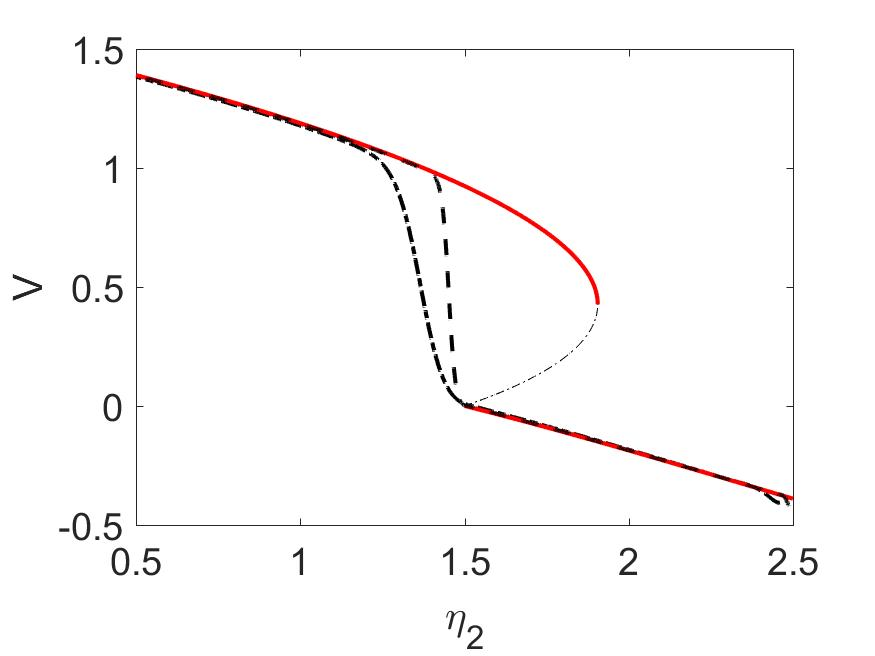
\includegraphics[width=\linewidth]{twoD/slow_bif_diagram.jpg}
  \caption{}
\end{subfigure}%
\begin{subfigure}{.5\textwidth}
  \centering
  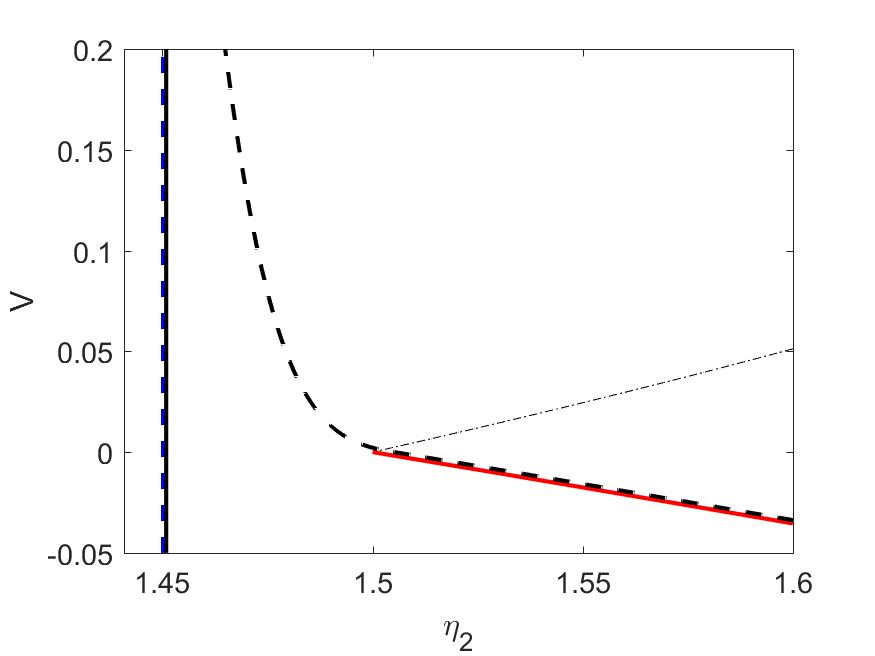
\includegraphics[width=\linewidth]{twoD/slow_bif_diagram_zoom.jpg}
  \caption{}
\end{subfigure}
\caption{In (a) the numerical solution (black dotted line) to \eqref{eq:twoD_canonical} is given with $\eta_1=4$, $\eta_3=.375$, and $\epsilon=.01$. In (b) a zoom in closer to the non-smooth bifurcation region where the blue vertical line is the prediction \eqref{eq:twoD_slow_tipping} against the black dotted vertical line which is the numerical tipping point.}
\label{fig:twoD_slow_Vnumerics}
\end{figure}

In figure~\ref{fig:twoD_slow_Vnumerics} an example of the slowly varying is given for a choice of $\epsilon$ in (a) and we zoom in around the non-smooth bifurcation in (b). Here we use the tipping criteria to be whenever $V>0.5$, this is large enough that the solution is going towards the upper branch indefinitely and is around the point of the smooth bifurcation. The effect of seeing a delay moving towards the upper branch in the $V$ solution causes a similar delay in $T$ seen in figure~\ref{fig:twoD_slow_Tnumerics}, where the delay causes the maximum value of $T$ to never be achieved. Here notice that after the tipping occurs, the numerical solution passes entirely over the unstable branch and even some of the upper stable branch before it resumes following closely.

\begin{figure}[H]
\centering
\begin{subfigure}{.5\textwidth}
  \centering
  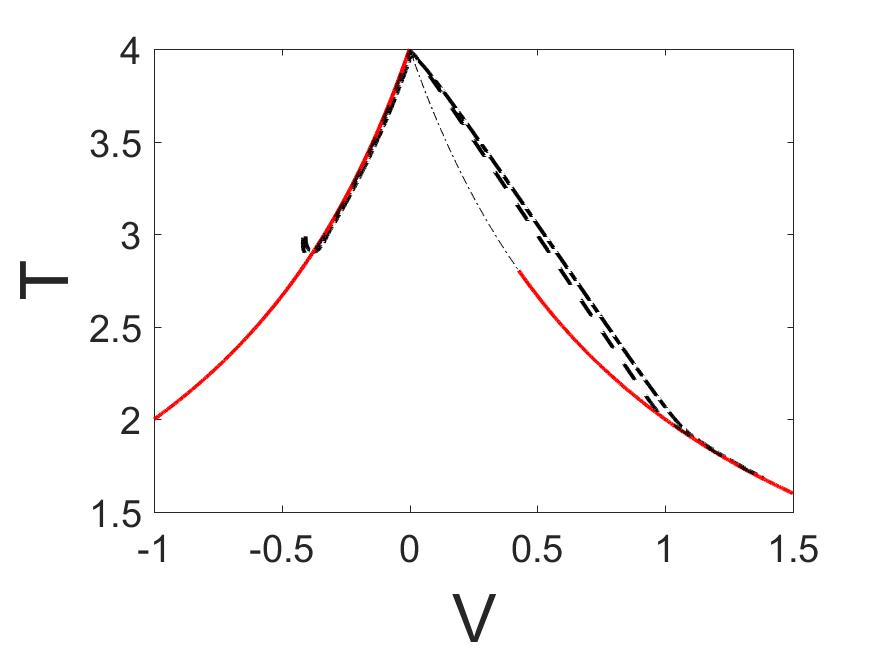
\includegraphics[width=\linewidth]{twoD/slow_bif_Tplot.jpg}
  \caption{}
\end{subfigure}%
\begin{subfigure}{.5\textwidth}
  \centering
  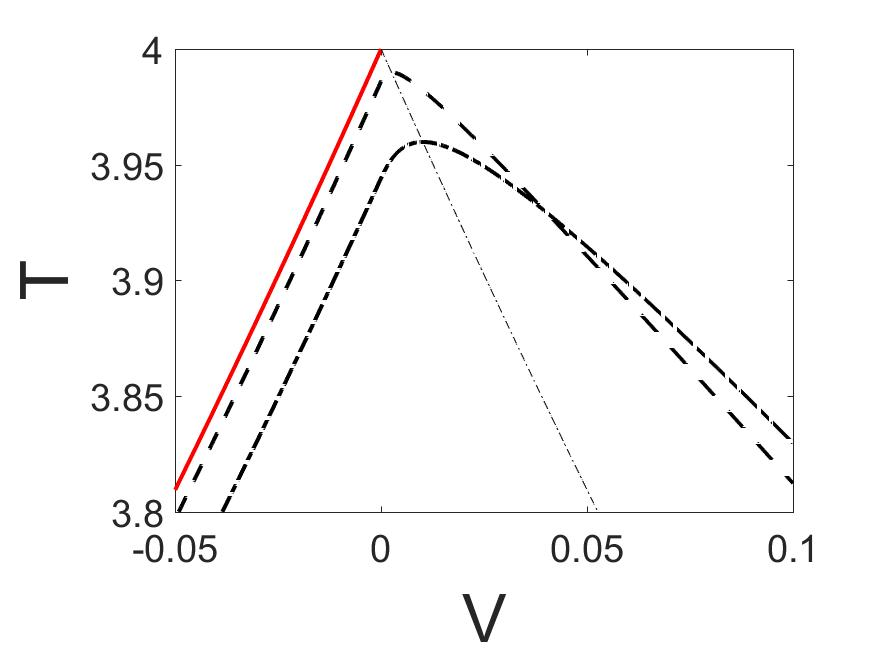
\includegraphics[width=\linewidth]{twoD/slow_bif_Tplot_zoom.jpg}
  \caption{}
\end{subfigure}
\caption{In (a) we have the numerical solution (black dotted) over the standard equilibrium plot for $V$ vs. $T$. In (b) a zoom of the bifurcation area.}
\label{fig:twoD_slow_Tnumerics}
\end{figure}

In figure~\ref{fig:twoD_slow_epscomp} we compare the numerical tipping to the predicted tipping in \eqref{eq:twoD_slow_tipping} over a range of epsilon. Here we see performance even better than in section \autoref{sec:oneD_slow} as even for relatively large $\epsilon$ the prediction has small error. This is an artifact of having a higher dimensional problem, where now two exponentials in \eqref{eq:twoD_slow_inneroriginal} are dominating the behavior of the solution in the $V>0$ region. As in \autoref{sec:oneD_slow}, the concavity of the predicted tipping against the numerical tipping match very well and we can expect the prediction to hold for reasonably small values of $\epsilon$.

\begin{figure}[H]
\centering
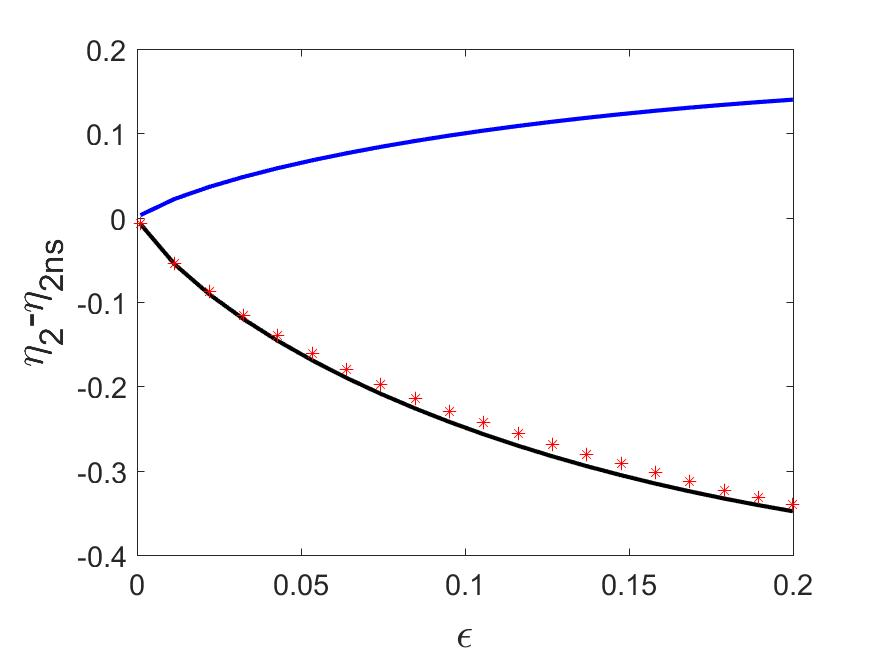
\includegraphics[width=\linewidth]{twoD/slow_epscomp.jpg}
\caption{The numerical tipping vs the estimate with $\eta_1=4$ and $\eta_3=\frac{3}{8}$. The tipping criteria is $V>.5$.}
\label{fig:twoD_slow_epscomp}
\end{figure}

\section{High Frequency Oscillatory Forcing}
\label{sec:twoD_highfreqosc}

It is a physical behavior of the THC to see oscillations occurring in the dynamics that is not originally encompassed by the Stommel model \cite{alley2003abrupt,huybers2005obliquity,marotzke2000abrupt,rahmstorf2000thermohaline,rahmstorf2002ocean,stastna2007box}. We choose to allow $\eta_1$ and $\eta_2$ to exhibit oscillatory behavior to account for this. As these parameters appear in both equations for $V$ and $T$, here we consider the canonical system \eqref{eq:twoD_canonical} with $A,B\sim O(1)$, $\Omega\gg 1$ and $\epsilon=0$ which is the purely oscillatory forcing problem. Under these conditions, we expect to find oscillations about some stable behavior; this stable behaior should act like the equilibria of a reduced inner problem. Thus our analysis must locate these equilibria for each variable up to the oscillations in order to find the bifurcation.

To begin our analysis, we note that there is behavior happening on multiple time scales, a 'slow' $t$ and 'fast' $R = \Omega t$. Following the multiple scales method, we consider $V(t)=V(t,R)$ and $T(t)=T(t,R)$ and substituting this into \eqref{eq:twoD_canonical}, we get the system

\begin{equation}\label{eq:twoD_osc_multiscaleouter}
\begin{aligned}
V_R+\Omega^{-1}V_t = & \Omega^{-1}\left(\eta_1-\eta_2+\eta_3(T-V)-T-V|V|+A\sin(R)\right),\\
T_R+\Omega^{-1}T_t = & \Omega^{-1}\left(\eta_1-T(1+|V|)+B\sin(R)\right).
\end{aligned}
\end{equation}

As per our typical approach to the non-smooth behavior, we follow the lower branch to isolate this dynamic. Thus we consider the system \eqref{eq:twoD_osc_multiscaleouter} with $V<0$

\begin{equation}\label{eq:twoD_osc_multiscaleouterlower}
\begin{aligned}
V_R+\Omega^{-1}V_t = & \Omega^{-1}\left(\eta_1-\eta_2+\eta_3(T-V)-T+V^2+A\sin(R)\right),\\
T_R+\Omega^{-1}T_t = & \Omega^{-1}\left(\eta_1-T(1-V)+B\sin(R)\right).
\end{aligned}
\end{equation}

From \eqref{eq:twoD_osc_multiscaleouterlower}, it makes sense to consider an asymptotic expansion for both $V$ and $T$ in terms of the small quantity that appears, $\Omega^{-1}$, with

\begin{equation}\label{eq:twoD_osc_outerexpansion}
\begin{aligned}
V(t,R)\sim V_0(t,R) +\Omega^{-1}V_1(t,R) +\Omega^{-2}V_2(t,R)+O(\Omega^{-3}),\\
T(t,R)\sim T_0(t,R) +\Omega^{-1}T_1(t,R) +\Omega^{-2}T_2(t,R)+O(\Omega^{-3}).
\end{aligned}
\end{equation}

Substituting \eqref{eq:twoD_osc_outerexpansion} into the system \eqref{eq:twoD_osc_multiscaleouterlower} gives

\begin{equation*}
\begin{aligned}
{V_0}_R+\Omega^{-1}{V_0}_t+\Omega^{-1}{V_1}_R+\ldots=&\begin{aligned}[t]\Omega^{-1}&(\eta_1-\eta_2+\eta_3(T_0-V_0)-T_0+V_0^2+A\sin(R))\\
+&\Omega^{-2}(\eta_3(T_1-V_1)-T_1+2V_1V_0)+\ldots
\end{aligned}\\
{T_0}_R+\Omega^{-1}{T_0}_t+\Omega^{-1}{T_1}_R+\ldots=&\begin{aligned}[t]  \Omega^{-1}&(\eta_1-T_0(1-V_0)+B\sin(R))\\
+&\Omega^{-2}(-T_1(1-V_0)+T_0V_1)+\ldots
\end{aligned}
\end{aligned}
\end{equation*}

Which we then find the following equations separated by order of $\Omega^{-1}$ with

\begin{align}
\label{eq:twoD_osc_outerO1}
O(1):\quad & \begin{cases}
	{V_0}_R =&  0, \\
	{T_0}_R =&  0,\\
\end{cases}\\
\label{eq:twoD_osc_outerO2}
O(\Omega^{-1}):\quad & \begin{cases}
	{V_1}_R+{V_0}_t = & \eta_1-\eta_2+\eta_3(T_0-V_0)-T_0+V_0^2+A\sin(R),\\
	 {T_1}_R +{T_0}_t =&  \eta_1-T_0(1-V_0)+B\sin(R),
\end{cases}\\
\label{eq:twoD_osc_outerO3}
O(\Omega^{-2}):\quad & \begin{cases}
	{V_2}_R+{V_1}_t = & \eta_3(T_1-V_1)-T_1+2V_0V_1,\\
	 {T_2}_R +{T_1}_t =&  -T_1(1-V_0)+T_0V_1.
\end{cases}
\end{align}

We learn from \eqref{eq:twoD_osc_outerO1} that both our leading order terms are purely dependent on the slow variable, $V_0=V_0(t)$, $T_0=T_0(t)$. But much like \autoref{sec:oneD_highfreqosc}, we must introduce a solvability condition on the resonant terms to be able to solve for the correction terms. This secures terms that are both consistent with one another as well as less than linear in their growth, making for a stable expansion. Here, we use the Fredholm alternative \eqref{eq:Fredholm} on \eqref{eq:twoD_osc_outerO2}-\eqref{eq:twoD_osc_outerO3} and search for the equilibrium solutions, the work for this can be found in \autoref{app:twoD}. This leads to the outer solution in original coordinates

\begin{equation}\label{eq:twoD_osc_outersoln}
\begin{aligned}
V\sim& V_0-\Omega^{-1} A\cos(\Omega t)+\dots\\
%\Omega^{-2}\left(V_2(t)+\left(A(\eta_3-2V_0)+B(1-\eta_3)\right)\sin(\Omega t)\right),\\
T\sim& T_0-\Omega^{-1} B\cos(\Omega t)+\ldots%\Omega^{-2}\left(T_2(t)+(1-V_0)B-T_0A)\sin(\Omega t)\right).
\end{aligned}
\end{equation}

Where $V_0$ and $T_0$ are the same equilibrium solutions from the static model in the introduction with

\begin{equation*} \label{eq:twoD_lowerleadingorder}
\begin{aligned}
T_0(V_0)=&\frac{\eta_1}{1-V_0},\\
0=\eta_1-\eta_2+\eta_3&(T_0(V_0)-V_0)-T_0(V_0)+V_0^2.
\end{aligned}
\end{equation*}

From the one-dimensional model in \autoref{sec:oneD_highfreqosc}, we discovered that in order to access the bifurcation we needed to scale both the coordinate $x$ as well as the parameter $\mu$ and analyze the behavior occurring around axis for $x=0$. Since we still have non-smooth behavior occurring at the axis $V=0$, we expect this approach to hold for the two-dimensional model as well. But the outer solution \eqref{eq:twoD_osc_outersoln} is too complex for us to search for when the assumptions of the asymptotic series break that would help find the appropriate scaling. Instead, a separate scales analysis analogous to  \autoref{sec:oneD_highfreqosc} leads to the following scaling

\begin{equation}\label{eq:twoD_osc_scales}
\begin{aligned}
V=&\Omega^{-1}X,\\
T=& \eta_1 +\Omega^{-1}Y,\\
\eta_2=&\eta_1\eta_3+\Omega^{-1} n.
\end{aligned}
\end{equation}

Substituting \eqref{eq:twoD_osc_scales} into \eqref{eq:twoD_canonical} leads to the following inner system

\begin{equation}\label{eq:twoD_osc_innersystem}
\begin{aligned}
\dot{X}=& -n+\eta_3(Y-X)-Y-\Omega^{-1}X|X| +\Omega A\sin(\Omega t),\\
\dot{Y}=& -\eta_1|X|-Y -\Omega^{-1}|X|Y +\Omega A \sin(\Omega t).
\end{aligned}
\end{equation}

Where we still see behavior on the same time scales in \eqref{eq:twoD_osc_innersystem}, the 'slow' $t$ and the 'fast' $R=\Omega t$. Considering both $X(t)=X(t,R)$ and $Y(t)=Y(t,R)$ gives the multiple scales inner system

\begin{equation}\label{eq:twoD_osc_innermulti}
\begin{aligned}
X_R+\Omega^{-1}X_t =& \Omega^{-1}\left(-n +\eta_3(Y-X)-Y\right)-\Omega^{-2}X|X|+A\sin(R),\\
Y_R+\Omega^{-1}Y_t =& \Omega^{-1}\left(-\eta_1|X|-Y\right)-\Omega^{-2}|X|Y+ B\sin(R).
\end{aligned}
\end{equation}

Once more, as we see the small quantity $\Omega^{-1}$ appearing in \eqref{eq:twoD_osc_innermulti}, then we choose an expansion of the form

\begin{equation}\label{eq:twoD_osc_innerexpan}
\begin{aligned}
X(t,R)\sim& X_0(t,R)+\Omega^{-1}X_1(t,R)+O(\Omega^{-2}),\\
Y(t,R)\sim& Y_0(t,R)+\Omega^{-1}Y_1(t,R)+O(\Omega^{-2}),
\end{aligned}
\end{equation}

where we then substitute \eqref{eq:twoD_osc_innerexpan} into \eqref{eq:twoD_osc_innermulti} to give the equation containing dynamics of all orders

\begin{equation*}
\begin{aligned}
{X_0}_R+\Omega^{-1}{X_0}_t+\Omega^{-1}{X_1}_R+\ldots=&\begin{aligned}[t]\Omega^{-1}&(-n+\eta_3(Y_0-X_0)-Y_0)+A\sin(R)\\
+&\Omega^{-2}(X_0|X_0+\Omega^{-1}X_1+\ldots|+\eta_3(Y_1-X_1)-Y_1)+\ldots
\end{aligned}\\
{Y_0}_R+\Omega^{-1}{Y_0}_t+\Omega^{-1}{Y_1}_R+\ldots=&\begin{aligned}[t]\Omega^{-1}&(-\eta_1|X_0+\Omega^{-1}X_1+\ldots|-Y_0)+B\sin(R)\\
+&\Omega^{-2}(-|X_0+\Omega^{-1}X_1+\ldots|Y_0-Y_1)+\ldots
\end{aligned}
\end{aligned}
\end{equation*}

We then separate the dynamics by their respective contribution to the solution, here by order of $\Omega^{-1}$, to find the following equations

\begin{align}
\label{eq:twoD_osc_innerO1}
O(1):\quad & \begin{cases}
	{X_0}_R =& A\sin(R), \\
	{Y_0}_R =& B\sin(R),\\
\end{cases}\\
\label{eq:twoD_osc_innerO2}
O(\Omega^{-1}):\quad & \begin{cases}
	{X_1}_R+{X_0}_t =& -n-\eta_3X_0-(1-\eta_3)Y_0, \\
	{Y_1}_R+{Y_0}_t =& -\eta_1|X_0|-Y_0.\\
\end{cases}
\end{align}

From \eqref{eq:twoD_osc_innerO1} we find that the leading order terms of \eqref{eq:twoD_osc_innerexpan} have the form in terms of the time scales

\begin{equation}\label{eq:twoD_osc_innerO1soln}
X_0=P_0(t)-A\cos(R),\quad Y_0=Q_0(t)-B\cos(R).
\end{equation}
 
Substituting \eqref{eq:twoD_osc_innerO1soln} into \eqref{eq:twoD_osc_innerO2}, we apply the Fredholm alternative \eqref{eq:Fredholm} to solve in terms of the separate time scales. This results in

\begin{equation}\label{eq:twoD_osc_innerintegral}
\begin{aligned}
{P_0}_t =& -n -\eta_3P_0-(1-\eta_3)Q_0,\\
{Q_0}_t =& -\frac{\eta_1}{2\pi}\int_0^{2\pi}|P_0-A\cos(R)|dR-Q_0.
\end{aligned}
\end{equation}

As we are concerned with finding the bifurcation, we search for the equilibrium solutions to \eqref{eq:twoD_osc_innerintegral} but we find a similar integral equation to the inner equation in \autoref{sec:oneD_highfreqosc}. This leads us to the similar two case argument. Case I: $|P_0(t)|\le -|A|$ which prevents the sign of the integrand from changing, and Case II: $|P_0(t)|<|A|$ where the integrand experiences the sign flipping and the integral has a non-trivial solution. These cases can be seen in figure~\ref{fig:twoD_osc_cases}.

\begin{figure}[H]
\centering
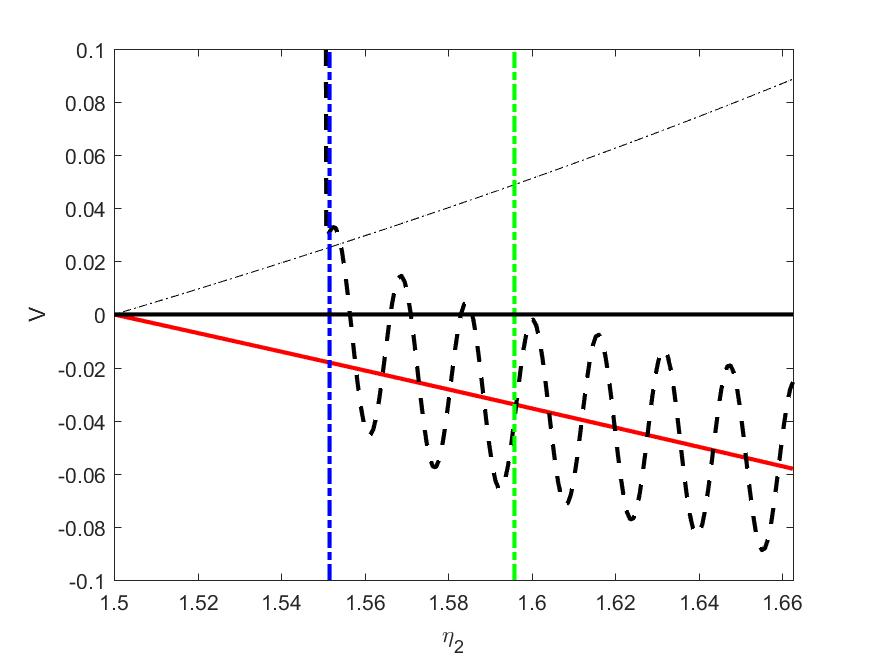
\includegraphics[scale=.25]{twoD/osc_cases.jpg}
\caption{Here we have the parameter ranges for Case I and Case II shown as the right most green vertical line and the bifurcation at the left blue vertical line respectfully.}
\label{fig:twoD_osc_cases}
\end{figure}

\subsection{Case I: $P_0(t)\le -|A|$}
\label{subsec:twoD_highfreqosc_caseI}

We call this the entirely below axis case; here with the size of the solution $X_0$ being far enough from the axis to see no bifurcating behavior. This case helps to simplify the integration in \eqref{eq:twoD_osc_innerintegral} but also helps us to determine when the solution begins to act differently. Here we use the equilibria to define a boundary between Case I and Case II. Under the conditions of this case, the system \eqref{eq:twoD_osc_innerintegral} simplifies to

\begin{equation}\label{eq:twoD_osc_caseIsystem}
\begin{aligned}
{P_0}_t(t) =& -n -\eta_3P_0(t)-(1-\eta_3)Q_0(t),\\
{Q_0}_t(t) =& \eta_1P_0(t)-Q_0(t).
\end{aligned}
\end{equation}

Solving for the equilibria in \eqref{eq:twoD_osc_caseIsystem} results in

\begin{equation*}
Q_0(P_0)=\eta_1P_0\quad,P_0=-\frac{n}{\eta_1(1-\eta_3)+\eta_3}. 
\end{equation*}

Together with these equilibria and with the condition of the case, $P_0(t)\le -|A|$, we find the parameter range that distinguishes between Case I and Case II in terms of our inner parameter, which we then rewrite in original coordinates with

\begin{equation}\label{eq:twoD_osc_boundary}
\begin{aligned}
n\ge& (\eta_1(1-\eta_3)+\eta_3)|A|,\\
\eta_2\ge&\eta_1\eta_3+ \frac{(\eta_1(1-\eta_3)+\eta_3)|A|}{\Omega}.
\end{aligned}
\end{equation}

So for values of $\eta_2$ less that the boundary given in \eqref{eq:twoD_osc_boundary}, we begin to see the oscillations crossing above the axis and hence use a separate case to deal with this behavior.

\subsection{Case II: $|P_0(t)|<|A|$}
\label{subsec:twoD_highfreqosc_caseII}

We call this the crossing case; here the solution is beginning to oscillate about the axis while the center of the oscillations approach the axis. With this behavior, we expect a bifurcation to occur in this region and thus we must find the equilibria for \eqref{eq:twoD_osc_innerintegral} that will help determine the location. While this problem is two-dimensional in nature, the integral in \eqref{eq:twoD_osc_innerintegral} is nearly identical to the integral of difficulty in \autoref{sec:oneD_highfreqosc}. So we may use the ideas of that section here to form an approximate solution. Thus, under the assumptions of this case, we fix a value of $P_0$ and integrate \eqref{eq:twoD_osc_innerintegral} over the regions where the integrand take the same sign with

\begin{equation*}
R_1=\arccos(P_0/A),\quad R_2=2\pi-\arccos(P_0/A).
\end{equation*}

We make the same assumption in \autoref{sec:oneD_highfreqosc} that the solution to \eqref{eq:twoD_osc_innerintegral} is negative for $P_0(t)$ the region $R\in[0,R_1]$ and alternates sign for the regions $R\in (R_1,R_2]$ and $R\in (R_2,2\pi]$. With this assumption, we also follow the same procedure of integrating over each region to get the exact form for \eqref{eq:twoD_osc_innerintegral} with

\begin{equation}\label{eq:twoD_osc_caseIIexact}
\begin{aligned}
{P_0}_t=&-n- \eta_3 P_0(t)-(1-\eta_3)Q_0,\\
{Q_0}_t=&-\frac{2\eta_1}{\pi}\left(\arcsin(P_0/A)P_0+\sqrt{A^2-P_0^2}\right)-Q_0.
\end{aligned}
\end{equation}

Although this is the explicit inner equation from \eqref{eq:twoD_osc_caseIIexact}, this is analytically too complex to find an explicit form for any bifurcating behavior and thus we use a second order Taylor approximation to find the solvable system

\begin{equation}\label{eq:twoD_osc_taylor}
\begin{aligned}
{P_0}_t=&-n -\eta_3 P_0-(1-\eta_3)Q_0,\\
{Q_0}_t=&-\frac{2\eta_1|A|}{\pi}-Q_0-\frac{\eta_1}{\pi|A|}P_0^2.
\end{aligned}
\end{equation}

Recalling that the equilibria will lead to the bifurcation, we solve \eqref{eq:twoD_osc_taylor} to give the inner solution. For simplicity, define $a=\frac{\eta_1}{\pi|A|}$, and $ c=\frac{2\eta_1|A|}{\pi}$,

\begin{equation}\label{eq:twoD_osc_equilibria}
\begin{aligned}
Q_0(P_0)=&-aP_0^2-c,\\
0=-n+\frac{2\eta_1(|A|}{\pi}&-\eta_3 P_0+\frac{\eta_1}{\pi |A|}P_0^2.
\end{aligned}
\end{equation}

Where the equation for $P_0$ in \eqref{eq:twoD_osc_equilibria} is a quadratic that would have two solutions, we recall the lower branch as being what we follow for this analysis, so we choose the negative solution with

\begin{equation}\label{eq:twoD_osc_innersolution}
P_0=\frac{\eta_3}{2a(1-\eta_3)}- \frac{1}{2a(1-\eta_3)}\sqrt{\eta_3^2+4a(1-\eta_3)(n-c(1-\eta_3))}.
\end{equation}

With the equilibrium for $P_0$ in \eqref{eq:twoD_osc_innersolution} containing a square root, this fails once the discriminant becomes negative. It is with this sudden failure that we have the bifurcation, here occurring for

\begin{equation*}
n_{osc} = \frac{\eta_1(1-\eta_3)|A|}{\pi}\left[2-\left(\frac{\pi\eta_3}{2\eta_1(1-\eta_3)}\right)^2\right].
\end{equation*}

Where we have the inner equilibria found, we write \eqref{eq:twoD_osc_innersolution} along with the oscillations as well as the oscillatory bifurcation in original coordinates

\begin{equation}\label{eq:twoD_osc_innersolnoriginal}
\begin{aligned}
V(t)\sim& \Omega^{-1}\left(P_0-A\cos(\Omega t)\right),\\
T(t)\sim& \eta_1-\Omega^{-1}\left(\frac{\eta_1}{\pi|A|}P_0^2+\frac{2\eta_1|A|}{\pi}+B\cos(\Omega t)\right),
\end{aligned}
\end{equation}

\begin{equation}\label{eq:twoD_osc_bifurcation}
{\eta_2}_{osc} = \eta_1\eta_3+\frac{\eta_1(1-\eta_3)|A|}{\pi\Omega}\left[2-\left(\frac{\pi\eta_3}{2\eta_1(1-\eta_3)}\right)^2\right].
\end{equation}

With \eqref{eq:twoD_osc_bifurcation} we have found the bifurcation induced with the addition of oscillatory forcing in the Stommel model. As we learned from the one-dimensional model in \autoref{sec:oneD_highfreqosc}, the effect of oscillatory forcing is early bifurcations. Our result in \eqref{eq:twoD_osc_bifurcation} agrees with this heuristic under the caveat that we restrict the parameters with 

\begin{equation*}
\eta_3 <\frac{2\sqrt{2}\eta_1}{\pi+2\sqrt{2}\eta_1},
\end{equation*}

which is the condition to guarantee the second term in \eqref{eq:twoD_osc_bifurcation} is positive. This restriction is reasonable as generally the parameters have the behaviors of $\eta_3<1$ and $\eta_3\ll \eta_1$ where the thermal variation is much larger in real ocean dynamics than the ratio of relaxation times.

In figure~\ref{fig:twoD_osc_Vnumerics} the numerical solution to \eqref{eq:twoD_canonical} for $V$ and a zoom of the solution around the numerical bifurcation is shown. The static bifurcation diagram is underlayed as well for comparison. We contrast the result in \eqref{eq:twoD_osc_bifurcation} to these numerics and find the bifurcation prediction from our analysis agrees in $V$. Notice that there is an early bifurcation for this problem, where certain values of the lower branch are never achieved.
In figure~\ref{fig:twoD_osc_Tnumerics} the numerical solution to \eqref{eq:twoD_canonical} for $T$ and a zoom in around the bifurcation is shown. Once more, the static bifurcation diagram is underlayed and we have two interesting features to note. Due to the early bifurcation in $V$, the maximum value of $T$ is never reached in (b). But due to the early bifurcation, there is a region of both the lower and the upper branch in $V$ that is never followed and we see that range being skipped over by the numerics in (a).

\begin{figure}[H]
\centering
\begin{subfigure}{.5\textwidth}
  \centering
  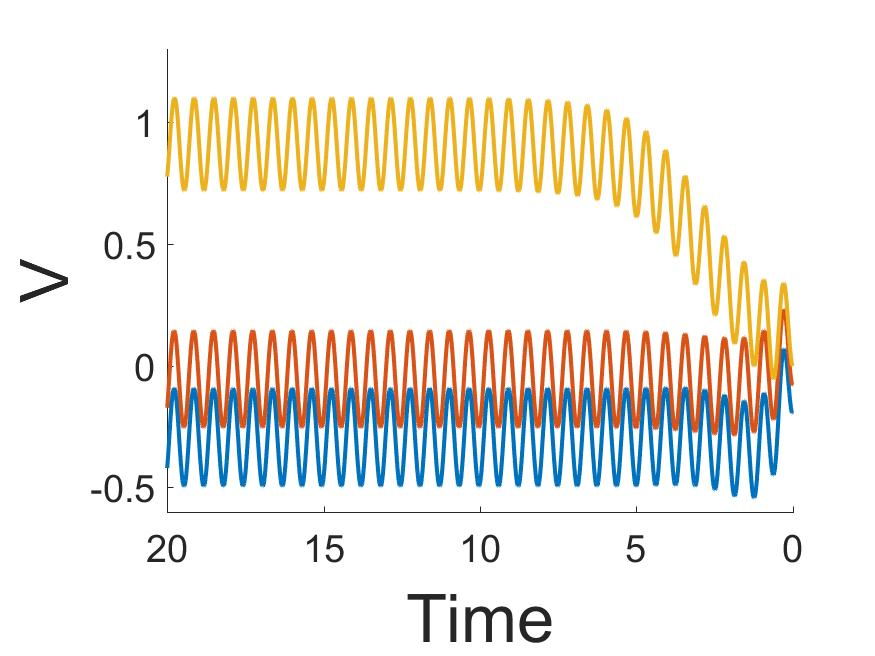
\includegraphics[width=\linewidth]{twoD/osc_Vtimeseries.jpg}
  \caption{}
\end{subfigure}%
\begin{subfigure}{.5\textwidth}
  \centering
  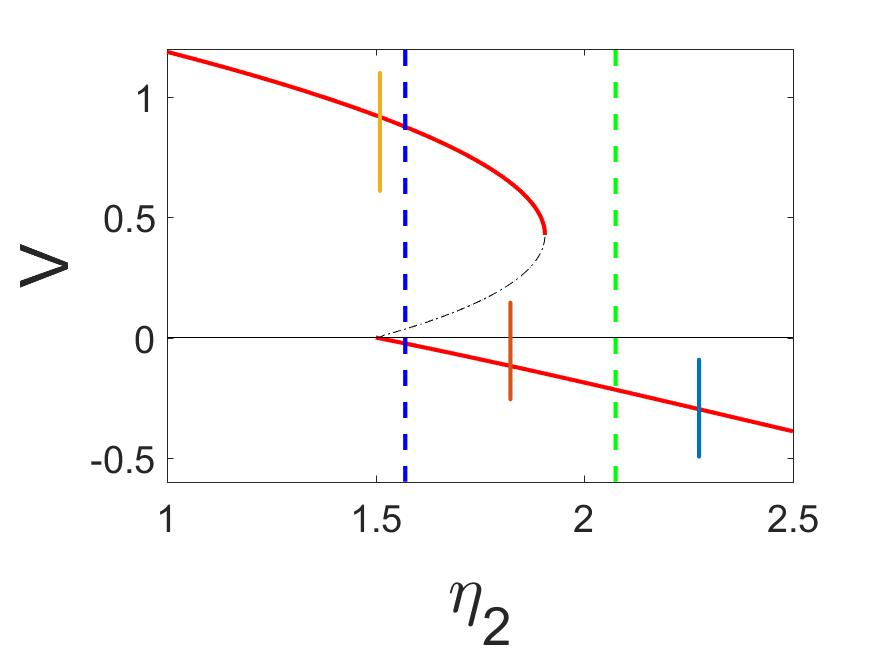
\includegraphics[width=\linewidth]{twoD/osc_bif_diagram.jpg}
  \caption{}
\end{subfigure}
\begin{subfigure}{.5\textwidth}
  \centering
  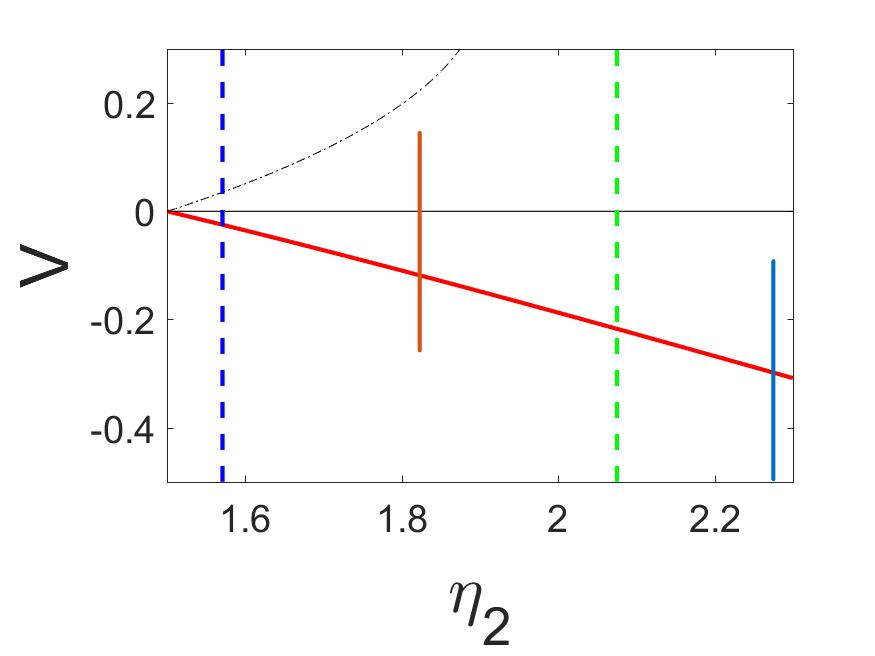
\includegraphics[width=\linewidth]{twoD/osc_bif_diagram_zoom.jpg}
  \caption{}
\end{subfigure}
\caption{In (a) the numerical time series solutions to \eqref{eq:twoD_canonical} is given with parameters in each qualitatively different case of $\eta_2$ with $\eta_1=4$, $\eta_3=.375$, $A=10$ and $\Omega = 10$. In (b) these same solutions are shown on the phase plane. In (c) a zoom in closer to the non-smooth bifurcation region where the blue vertical line is the prediction \eqref{eq:twoD_slow_tipping} against the black dotted vertical line which is the numerical bifurcation.}
\label{fig:twoD_osc_Vnumerics}
\end{figure}

\begin{figure}[H]
\centering
\begin{subfigure}{.5\textwidth}
  \centering
  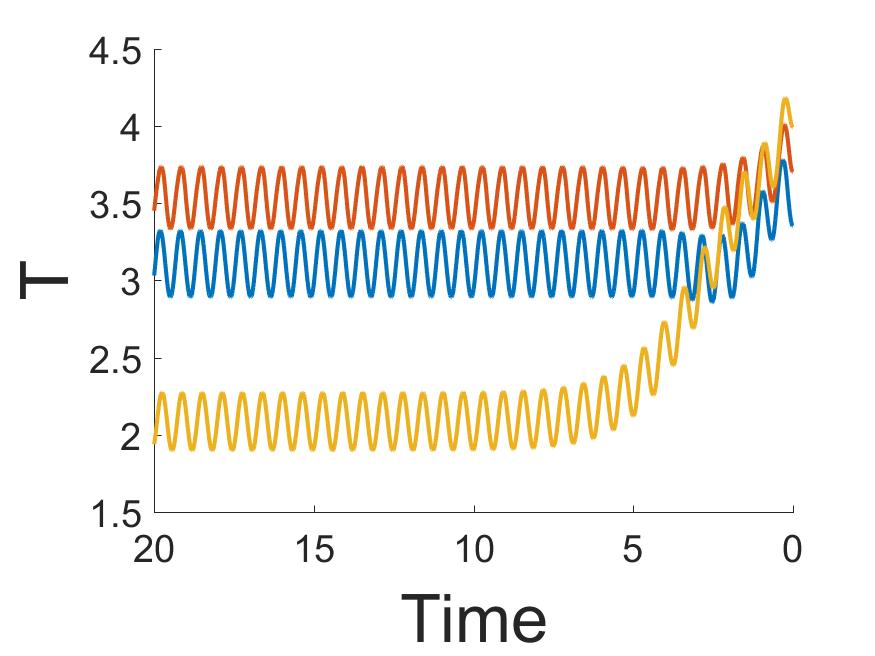
\includegraphics[width=\linewidth]{twoD/osc_Ttimeseries.jpg}
  \caption{}
\end{subfigure}%
\begin{subfigure}{.5\textwidth}
  \centering
  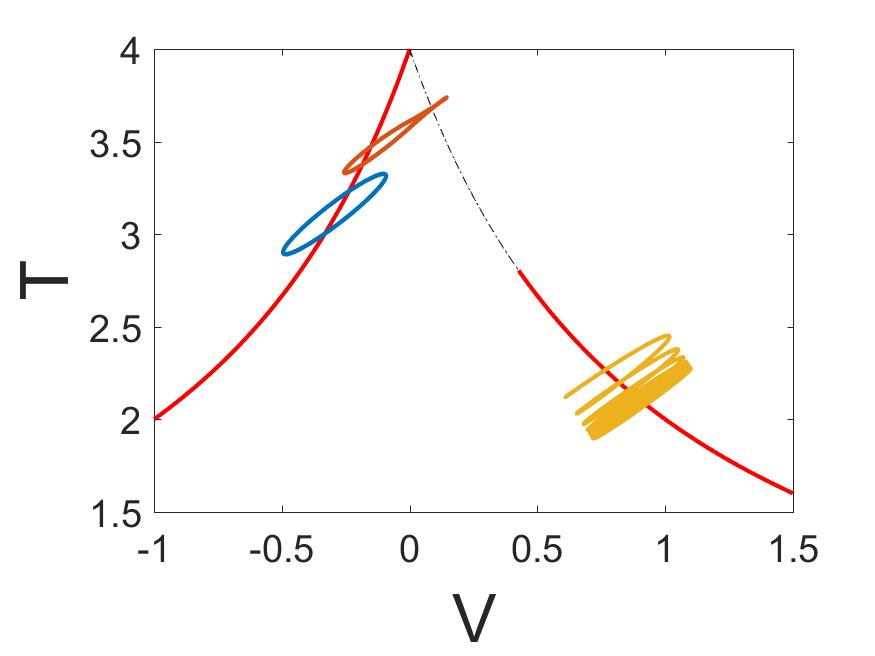
\includegraphics[width=\linewidth]{twoD/osc_bif_Tplot.jpg}
  \caption{}
\end{subfigure}
\begin{subfigure}{.5\textwidth}
  \centering
  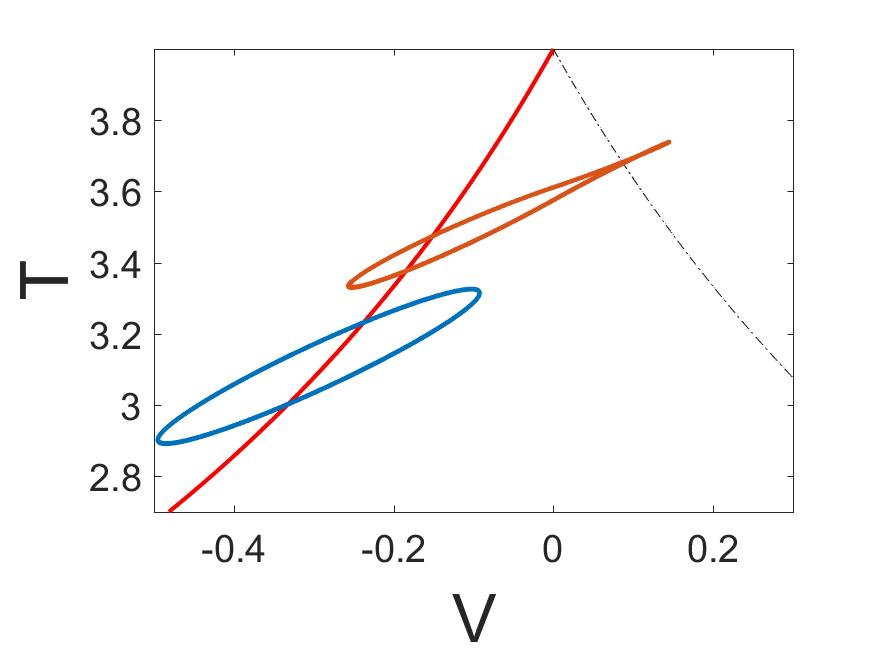
\includegraphics[width=\linewidth]{twoD/osc_bif_Tplot_zoom.jpg}
  \caption{}
\end{subfigure}
\caption{In (a) we have the numerical time series solutions for a qualitatively different cases of $\eta_2$. In (b) we plot these solutions over the standard equilibrium plot for $V$ vs. $T$. In (c) a zoom of the bifurcation area.}
\label{fig:twoD_osc_Tnumerics}
\end{figure}

To evaluate the performance of this prediction, we compare \eqref{eq:twoD_osc_bifurcation} to the numerical tipping criteria over a range of $\Omega^{-1}$. In figure~\ref{fig:twoD_osc_epscomp} we allow for this range to be $\Omega^{-1}\in (0,.5)$. For small values, the two agree very well and as we expect, they begin to diverge once the values of $\Omega^{-1}$ become too large from the assumption that $\Omega\gg 1$ and the asymptotics cannot capture the behavior for low frequency oscillations. But under our assumptions, the prediction is performing quite well and resembles the performance of \autoref{sec:oneD_highfreqosc}.

\begin{figure}[H]
\centering
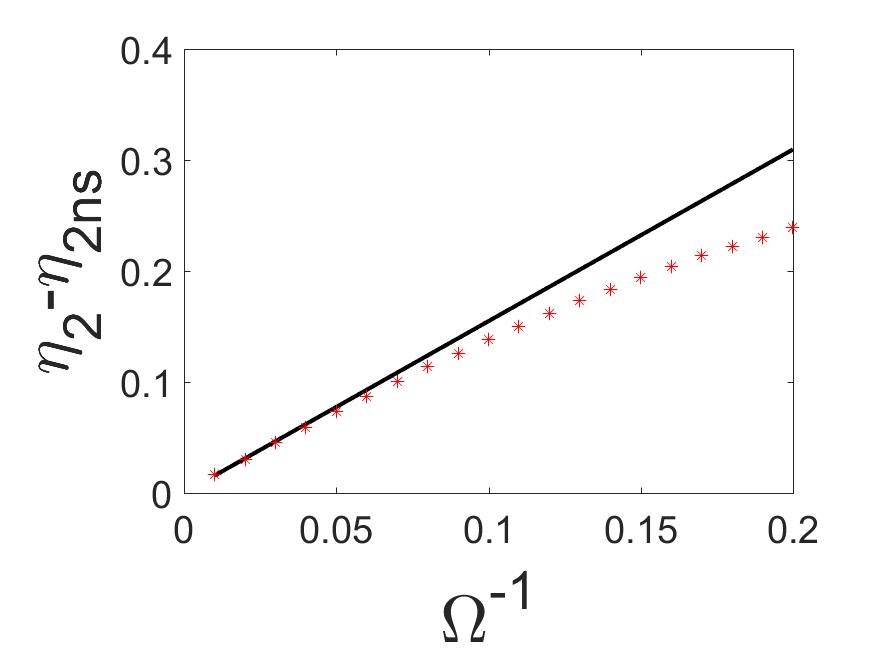
\includegraphics[scale=.25]{twoD/osc_Omegacomp.jpg}
\caption{The numerical tipping vs the estimate with $\eta_1=4$ and $\eta_3=\frac{3}{8}$. The tipping criteria is $V>.5$.}
\label{fig:twoD_osc_epscomp}
\end{figure}

\subsection{Stability}

Although the eigenvalues from \autoref{sec:twoD_slow} apply here, since we have a non-autonomous system when $A\not=0$, we must approach the stability with a linearized form about the equilibria much like in \autoref{sec:oneD_highfreqosc}. To do this, recall from our analysis that we found the system

\begin{equation}\label{eq:twoD_osc_stabilityequation}
\begin{aligned}
{P_0}_t =& -n -\eta_3 P_0-(1-\eta_3)Q_0,\\
{Q_0}_t =& -\frac{\eta_1}{2\pi}\int_0^{2\pi}|P_0-A\cos(R)|\, dR - Q_0.
\end{aligned}
\end{equation}

We must consider the stability of solutions over the relative sizes of $P_0(t)$ with Case I: $P_0(t)\le -|A|$ and Case II: $|)_0(t)|\le |A|$.

\subsubsection{Case I: $v_0(t)\le -|A|$}

From the analysis, we called this case the entirely below-axis case where the solution spends most of its time away from the axis $V=0$. We expected this case to be entirely controllable and thus we should see stability here. Under these conditions, the inner equation \eqref{eq:twoD_osc_stabilityequation} simplifies to a much simpler equation

\begin{equation}\label{eq:twoD_osc_stability_caseI_fullinner}
\begin{aligned}
{P_0}_t =& -m -\eta_3 P_0-(1-\eta_3)Q_0,\\
{Q_0}_t =& \eta_1 P_0 - Q_0.
\end{aligned}
\end{equation}

The equilibria of \eqref{eq:twoD_osc_stability_caseI_fullinner} is found with $Q_0(P_0)=\eta_1 P_0$, and thus we find the following one-dimensional equation and equilibrium

\begin{equation}\label{eq:twoD_osc_stability_caseI_red}
{P_0}_t = -n -(\eta_3 +(1-\eta_3))Q_0=f(P_0),\quad Z^0 = -\frac{n}{\eta_3+\eta_1(1-\eta_3)}.
\end{equation}

Now we consider a simple linear perturbation about this equilibrium with $P_0(t)= Z^0+U(t)$ where $\lVert U(t) \rVert \ll 1$. Our standard Taylor expansion about this equilibrium results in

\begin{equation}\label{eq:twoD_osc_stability_caseI_perteq}
\begin{aligned}
f(P_0)=&f(Z^0)+f_{P_0}(Z^0)(P_0-Z^0)+O((P_0-Z^0)^2),\\
U_t =& -(\eta_3+\eta_1(1-\eta_3))U + O(\lVert U\rVert ^2).
\end{aligned}
\end{equation}

From \eqref{eq:twoD_osc_stability_caseI_perteq} we now conclude the equilibrium $Z^0$ is hyperbolic and asymptotically stable due to the exponential decay in perturbations. Thus we find that no tipping will occur for this case, and from the analysis, this holds true until for the parameter range of $\eta_2$ from \eqref{eq:twoD_osc_boundary}

\begin{equation*}
\eta_2 \ge \eta_1\eta_3 +\frac{(\eta_3+\eta_1(1-\eta_3))|A|}{\Omega}.
\end{equation*}


\subsubsection{Case II: $|P_0(t)|<|A|$}

We called this case the crossing case and here the solution experiences all of the non-smooth behavior when it crosses $V=0$. We expect the stability to fail under these conditions and we discovered in the analysis that the crossing pattern caused the system \eqref{eq:twoD_osc_stabilityequation} to behave like

\begin{equation}\label{eq:twoD_osc_stability_caseII_full}
\begin{aligned}
{P_0}_t =& -n-\eta_3 P_0-(1-\eta_3)Q_0,\\
{Q_0}_t =& -\frac{2\eta_1|A|}{\pi}-\frac{\eta_1}{\pi |A|}P_0^2-Q_0.
\end{aligned}
\end{equation}

As we search for the equilibria of \eqref{eq:twoD_osc_stability_caseII_full}, we find the equilibrium for $Q_0$ in terms of $P_0$  

\begin{equation*}
Q_0(P_0)=-\frac{2\eta_1|A|}{\pi}-\frac{\eta_1}{\pi |A|}P_0^2
\end{equation*}

which then gives the following inner equation with the negatively chosen equilibrium for $P_0$

\begin{equation}\label{eq:twoD_osc_stability_caseII_inner}
\begin{aligned}
{P_0}_t=&-n+\frac{2\eta_1(|A|}{\pi}-\eta_3 P_0+\frac{\eta_1}{\pi |A|}P_0^2=f(P_0),\\
Z^0=&\frac{\pi |A|}{2\eta_1(1-\eta_3)}\left(\eta_3-\sqrt{n-n_{\text{osc}}}\right).
\end{aligned}
\end{equation}

For simplicity we write the argument of the square root in terms of oscillatory bifurcation we found in the analysis with \eqref{eq:twoD_osc_bifurcation}. We now consider a simple linear perturbation about this equilibrium in \eqref{eq:twoD_osc_stability_caseII_inner} with $P_0(t)=Z^0+U(t)$ where $\lVert U(t)\rVert\ll 1$. The standard Taylor expansion about the equilibrium is thus

\begin{equation}\label{eqLtwoD_osc_stability_caseII_perturb}
\begin{aligned}
f(P_0)=&f(Z^0)+f_{P_0}(Z^0)(P_0-Z^0)+O((P_0-Z^0)^2),\\
U_t=&\left(-\eta_3+\frac{2\eta_1(1-\eta_3)}{\pi |A|}Z^0\right)U,\\
U_t=&- \sqrt{n-n_{\text{osc}}}U.
\end{aligned}
\end{equation}

Thus with \eqref{eqLtwoD_osc_stability_caseII_perturb} we learn that the perturbations $U(t)$ decay exponentially as long as the square-root is non-zero and makes sense. Thus we have that $Z^0$ is a hyperbolic and asymptotically stable equilibrium for $P_0$ and thus we find stability in $Q_0$ as well. This gives stability for this region but we lose this stability once the square-root becomes zero, here when

\begin{equation*}
n_{osc} = \frac{\eta_1(1-\eta_3)|A|}{\pi}\left[2-\left(\frac{\pi\eta_3}{2\eta_1(1-\eta_3)}\right)^2\right].
\end{equation*}

This says the equilibrium $Z^0$ at this point is non-hyperbolic which is indicative of a bifurcation. This is in agreement with out analysis and thus we can say that the value found in \eqref{eq:twoD_osc_bifurcation} is the bifurcation under the oscillatory forcing.


\section{Slow Variation with Oscillatory Forcing}
\label{sec:twoD_slowosc}

With the one-dimensional model solved and both the slowly varying and high oscillatory two-dimensional components analyzed, we have all of the tools needed to analyze the full system \eqref{eq:twoD_canonical} with both $\epsilon \ll 1$ and $A,B\sim O(1)$ simultaneously. This is the most general setting we discuss in this paper where we account for both a slowly varying $\eta_2$ that leads to abrupt changes seen in \cite{alley2003abrupt,marotzke2000abrupt,rahmstorf2000thermohaline} as well as oscillatory forcing in both equations in \eqref{eq:twoD_canonical} seen in \cite{roberts2017relaxation,huybers2005obliquity}. We care to find the interaction of mechanisms in the physical Stommel model. Under the framework of slowly varying parameters we expect to find tipping instead of a bifurcation and hence our method for finding the tipping point follows a mixture of both \autoref{sec:twoD_slow} and \autoref{sec:twoD_highfreqosc}. This procedure dictates that we search for inner behavior about the non-smooth bifurcation and to do so we need to solve the inner equation and estimate when this solution becomes uncontrollable. Ultimately, we provide a realistic solution for where the abrupt change from the lower stable branch to the upper occurs in the full two-dimensional Stommel model.

To begin, we take our standard approach of following the lower branch towards the non-smooth behavior with $V<0$ in \eqref{eq:twoD_canonical} which gives the following system  

\begin{equation}\label{eq:twoD_slowosc_outereqs}
 \begin{aligned}
   \dot{V} & =  \eta_1-\eta_2-T+\eta_3(T-V)+V^2+A\sin(\Omega t), \\
   \dot{T} & =  \eta_1-T(1-V)+B\sin(\Omega t),  \\
  \dot{\eta_2}  & =  -\epsilon.
  \end{aligned}
\end{equation}

Much like in \autoref{sec:oneD_slowosc}, we assume there is a generic polynomial relationship between the frequency of our problem and the slow variation, $\Omega = \epsilon^{-\lambda}$ with strength parameter $\lambda>0$. It is this assumption that helps us to find the interaction between the slowly varying parameter and fast oscillations in the tipping. We notice in \eqref{eq:twoD_slowosc_outereqs} that there is behavior on a slow scale in $\eta_2(t)$ and on a fast scale in $\sin(\Omega t)$, so this suggests a multiple scales approach with 'slow' time $\tau = \epsilon t$ and 'fast' time $R=\epsilon^{-\lambda}t$. These scales cause \eqref{eq:twoD_slowosc_outereqs} to take the form

\begin{equation}\label{eq:twoD_slowosc_multiouter}
 \begin{aligned}
V_R+\epsilon^{\lambda+1}V_\tau & = \epsilon^{\lambda} \left(\eta_1-\eta_2-		T+\eta_3(T-V)+V^2+A\sin(R)\right), \\
T_R+\epsilon^{\lambda+1}T_\tau & = \epsilon^{\lambda}\left( \eta_1-T(1-		  V)+B\sin(R)\right),  \\
	{\eta_2}_\tau  & =  -1.
\end{aligned}
\end{equation}
  
From these multiple-scaled outer equations in \eqref{eq:twoD_slowosc_multiouter}, we find an asymptotic expansion in terms of our small recurring quantity $\epsilon^\lambda$ to be a good choice for separating the dynamics by order. But we must consider both multiples of $\lambda$ as well as integer powers as we have not specified the range of $\lambda$ and both could be significant, thus our expansion is

\begin{equation}\label{eq:twoD_slowosc_outerexpansion}
	\begin{aligned}
		V(\tau,R)\sim& V_0(\tau,R)+\epsilon^\lambda 	V_1(\tau,R)+O(\epsilon^{2\lambda},\epsilon^{\lambda+1}),\\
        T(\tau,R)\sim& T_0(\tau,R)+\epsilon^\lambda T_1(\tau,R)+O(\epsilon^{2\lambda},\epsilon^{\lambda+1}).
	\end{aligned}
\end{equation}

Which substituting \eqref{eq:twoD_slowosc_outerexpansion} into \eqref{eq:twoD_slowosc_multiouter} results in the governing dynamics for all orders of $\epsilon$ with

\begin{equation*}
\begin{aligned}
{V_0}_R+\epsilon^{\lambda+1}{V_0}_\tau+\epsilon^\lambda {V_1}_R+\ldots=&\begin{aligned}[t]&
\epsilon^\lambda \left(\eta_1-\eta_2-T+\eta_3(T_0-V_0)+V_0^2+A\sin(R)\right)\\
&+\epsilon^{2\lambda}\left(-\eta_3 V_1-(1-\eta_3)T_1+2V_0V_1\right)+\ldots
\end{aligned}\\
{T_0}_R+\epsilon^{\lambda+1}{T_0}_\tau+\epsilon^\lambda {T_1}_R+\ldots=&\begin{aligned}[t]&
\epsilon^\lambda\left( \eta_1-T_0(1-V_0)+B\sin(R)\right)\\
&+\epsilon^{2\lambda}\left(-T_1+T_0V_1+T_1V_0\right)+\ldots
\end{aligned}
\end{aligned}
\end{equation*}

Here we consider the next order in \eqref{eq:twoD_slowosc_outerexpansion} to be $O(\epsilon^{2\lambda})$ as the equations at $O(\epsilon^{\lambda+1})$ and $O(\epsilon^{2\lambda})$ result in the same information, so it does not matter whether we consider a $\lambda$ value that would cause $O(\epsilon^{2\lambda})$ to come before $O(\epsilon^{\lambda+1})$ or vice-versa. With this in mind, we find the following sets of equations at each order

\begin{align}
\label{eq:twoD_slowosc_outerO1}
O(1):\quad & \begin{cases}
	{V_0}_R =&  0, \\
	{T_0}_R =&  0,\\
\end{cases}\\
\label{eq:twoD_slowosc_outerO2}
O(\epsilon^\lambda):\quad & \begin{cases}
	{V_1}_R = & \eta_1-\eta_2(\tau) +\eta_3(T_0-V_0)-T_0+V_0^2+A\sin(R),\\
	{T_1}_R =&  \eta_1-T_0(1-V_0)+B\sin(R),
\end{cases}\\
\label{eq:twoD_slowosc_outerO3}
O(\epsilon^{2\lambda}):\quad & \begin{cases}
	{V_2}_R+\epsilon^{1-\lambda}{V_0}_\tau = & \eta_3(T_1-V_1)-T_1+2V_0V_1,\\
	{T_2}_R +\epsilon^{1-\lambda}{T_0}_\tau =&  -T_1(1-V_0)+T_0V_1,
\end{cases}
\end{align}

From \eqref{eq:twoD_slowosc_outerO1} the leading order terms in our expansion are purely slow dependent, $V_0=V_0(\tau)$ and $T_0=T_0(\tau)$. This allows the solutions of \eqref{eq:twoD_slowosc_outerO2} and \eqref{eq:twoD_slowosc_outerO3} to be found, the work for this is found in \autoref{app:twoD}. This results in the following outer solutions 

\begin{equation}\label{eq:twoD_slowosc_outersoln}
\begin{aligned}
V\sim& V_0 + \frac{\epsilon({V_0}_\tau(1-V_0)+(1-\eta_3){T_0}_\tau)}{(1-\eta_3)T_0+(2V_0-\eta_3)(1-V_0)}-\epsilon^\lambda A \cos(\Omega t),\\
T\sim& T_0 + \frac{\epsilon {T_0}_\tau}{1-V_0}-\frac{\epsilon T_0({V_0}_\tau(1-V_0)+(1-\eta_3){T_0}_\tau)}{(1-\eta_3)T_0(1-V_0)+(2V_0-\eta_3)(1-V_0)^2}-\epsilon^\lambda B \cos(\Omega t),
\end{aligned}
\end{equation}

where $V_0$ and $T_0$ are the same leading order solutions from the slowly varying Stommel model in \autoref{sec:twoD_slow}. Unfortunately the common theme of the two-dimensional model is that these outer solutions are too complex to see directly when an inner scaling is required so we perform a separate scale analysis analogous to that of \autoref{sec:oneD_slowosc} to find the appropriate inner scaling.

We make the assumption that the inner scaling for both $V$ and $T$ are the same which just makes this calculation slightly easier, but this isn't necessary to arrive at the same conclusion. Hence we chose a general scaling about the bifurcation point $(V,T,\eta_2)=(0,\eta_1,\eta_1\eta_3)$ with

\begin{equation}\label{eq:twoD_slowosc_general_scaling}
V=\epsilon^\alpha X, \quad T=\eta_1+\epsilon^\alpha Y ,\quad \eta_2(t)=\eta_1\eta_3+\epsilon^\beta n(t),
\end{equation}

where both $\alpha>0$ and $\beta>0$ allow for this to be an inner scaling. Applying the scalings in \eqref{eq:twoD_slowosc_general_scaling} to the full two-dimensional model \eqref{eq:twoD_canonical} gives

\begin{equation}\label{eq:twoD_slowosc_innerscaled}
\begin{aligned}
\epsilon^\alpha \dot{X}=& -\epsilon^\beta n(t)-\epsilon^\alpha (X+(1-\eta_3)Y) - \epsilon^{2\alpha}X|X| +A\sin(\epsilon^{-\lambda}t),\\
\epsilon^\alpha \dot{Y}=&-\epsilon^\alpha(\eta_1|X|+Y)+\epsilon^{2\alpha}|X|Y +B\sin(\epsilon^{-\lambda} t)\\
\dot{n}=&-\epsilon^{1-\beta}.
\end{aligned}
\end{equation}

From \eqref{eq:twoD_slowosc_innerscaled} it is apparent that fast behavior is still occurring on different time scales and to truly flesh out the particular choice in $\alpha$, we then take a multiple scales approach to capture the 'fast' behavior with scales $t$ and $R=\epsilon^{-\lambda}t$. Also note that we choose to have the 'slow' behavior has been moved into regular time with the scalings we applied to the space variables. This choice comes with the ambiguity in $\beta$ and is discussed further below. Applying the multiple scales in \eqref{eq:twoD_slowosc_innerscaled} results in

\begin{equation}\label{eq:twoD_slowosc_innergeneral}
\begin{aligned}
\epsilon^{\alpha-\lambda} X_R+\epsilon^{\alpha}X_t=& -\epsilon^{\beta}n(t)-\epsilon^{\alpha}(X+(1-\eta_3)Y)-\epsilon^{2\alpha}X|X|+A\sin(R),\\
\epsilon^{\alpha-\lambda}Y_R + \epsilon^{\alpha}Y_t =&- \epsilon^\alpha(\eta_1|X|+Y)-\epsilon^{2\alpha}|X|Y +B\sin(R)\\
n_t=&-\epsilon^{1-\beta}.
\end{aligned}
\end{equation}

Here we balance the leading order terms in each equation of \eqref{eq:twoD_slowosc_innergeneral}, $\epsilon^{\alpha-\lambda}X_R$ and $A\sin(R)$ as well as $\epsilon^{\alpha-\lambda}Y_R$ with $B\sin(R)$, which gives us that $\alpha=\lambda$ and confirms that the scales for each variable are the same. The scaling for $\eta_2$ has still yet to be determined and could have multiple possibilities depending on $\lambda$, but due to this choice in $\alpha$ we expect the oscillatory term to persist in the inner asymptotic expansion of \eqref{eq:twoD_canonical} regardless of choice in $\lambda$ and we have an effective means of tracking this behavior with this scaling.

We now consider the scales $t$ and $R=\epsilon^{-\lambda}t$ on the canonical system \eqref{eq:twoD_canonical} along with the general scaling on $\eta_2$ which gives

\begin{equation}\label{eq:twoD_slowosc_general_outermulti}
\begin{aligned}
V_R+\epsilon^{\lambda}V_t =& -\epsilon^{\lambda+\beta}n(t)-\epsilon^{\lambda}(\eta_1-\eta_1\eta_3+\eta_3(T-V)-T-V|V|+A\sin(R)),\\
T_R+\epsilon^{\lambda}T_t =& \epsilon^\lambda(\eta_1-T(1+|V|)+B\sin(R)),\\
n_t =&-\epsilon^{1-\beta}.
\end{aligned}
\end{equation}

We learned in \autoref{sec:oneD_slowosc} that the analysis from here depends on the relative size of the slow variation with respects to the oscillations. The distinction in these behaviors are when $\lambda\le1$ where a mixture between the slow variation and oscillations occur or $\lambda>1$ where the slow variation dominates the solution. We then consider a separate asymptotic expansion for the following Case I: $\lambda\le 1$ and Case II: $\lambda >1$ to find an accurate classification of behavior for the full two-dimensional Stommel model.

\subsection{Case I: $\lambda \le 1$}

We call this the mixed effects case where there is significant influence from both slow variation and fast oscillations due to the size of $\lambda$. Under this range for $\lambda$, there are two choices for the scaling on $\eta_2$, $\beta=1$ or $\beta=\lambda$. But we are unsure whether there should be integer powers in an asymptotic expansion due to the uncertainty of the scale $\beta$. Thus we choose a rather general expansion with

\begin{equation}\label{eq:twoD_slowosc_caseI_expansion}
\begin{aligned}
V(t,R)\sim& \epsilon^{\lambda} X_0(t,R)+\epsilon^q X_1(t,R)+\ldots\\
T(t,R)\sim& \eta_1+\epsilon^{\lambda} Y_0(t,R)+\epsilon^q Y_1(t,R)+\ldots
\end{aligned}
\end{equation}

with $q>\lambda$ to be consist with our analysis thus far. Substituting \eqref{eq:twoD_slowosc_caseI_expansion} into \eqref{eq:twoD_slowosc_general_outermulti} then gives the governing dynamics for this case

\begin{equation*}
\begin{aligned}
 {X_0}_R+\epsilon^{\lambda}{X_0}_t+\epsilon^{q-\lambda} {X_1}_R\ldots={} & -\epsilon^{\beta}n(t)-\epsilon^{\lambda} (\eta_3X_0+(1-\eta_3)Y_0) \\
&-\epsilon^{2\lambda}(X_0+\epsilon^{q-\lambda} X_1+\ldots)|X_0+\epsilon^{q-\lambda} X_1+\ldots|\\
& - \epsilon^{q}(\eta_3X_1+(1-\eta_3)Y_1) + A\sin(R) +\ldots
\end{aligned}
\end{equation*}

\begin{equation*}
\begin{aligned}
{Y_0}_R+\epsilon^{\lambda}{Y_0}_t+\epsilon^{q-\lambda} {Y_1}_R+\ldots= &-\epsilon^\lambda(\eta_1| X_0 +\epsilon^{q-\lambda} X_1+\ldots|+ Y_0+\epsilon^{q-\lambda} Y_1+\ldots)\\
&+\epsilon^{2\lambda}|X_0 +\epsilon^{q-\lambda} X_1+\ldots|(Y_0+\epsilon^{q-\lambda} Y_1+\ldots)\\
&+ B\sin (R)+\ldots
\end{aligned}
\end{equation*}

Where we now separate by the distinct orders of $\epsilon$ to find the following equations at each order

\begin{align} \label{eq:twoD_slowosc_caseI_O1}
O(1):\, &\begin{cases}
	{X_0}_R =&  A\sin(R), \\
	{Y_0}_R =&  B\sin(R),\\
\end{cases}\\ \label{eq:twoD_slowosc_caseI_O2}
O(\epsilon^\lambda): \, & \begin{cases}
	\epsilon^{q-2\lambda}{X_1}_R+{X_0}_t =&  -\epsilon^{\beta-\lambda} n(t) -\eta_3 X_0-(1-\eta_3)X_0, \\
	\epsilon^{q-2\lambda}{Y_1}_R+{Y_0}_t =&  -\eta_1|X_0|-Y_0.\\
\end{cases}
\end{align}

We learn from \eqref{eq:twoD_slowosc_caseI_O2} that $q= 2\lambda$ prevents terms from being unbalanced, which implies that $\lambda> \frac{1}{2}$ for an expansion to be found, otherwise we would need to include the quadratic terms at $O(\epsilon^\lambda)$ and our equations would be too complicated to solve analytically. This $q$ also suggests that there is no need for integer powers in the expansion \eqref{eq:twoD_slowosc_caseI_expansion} and all behavior is captures by the interaction between the the slow variation and frequency, $\epsilon^\lambda$. Since there is a choice in the scaling for $\eta_2$ where $\beta=\lambda$ or $\beta=1$ we must choose here to dictate the future of the analysis. The advantage to choosing $\beta=\lambda$ is that these inner equations are rather simple, but the slow variation is still small. On the other hand, $\beta=1$ keeps a small coefficient on the parameter but makes the slow variation simple. Both of these choices result in the same equations, so here we choose $\beta=1$ for simplicity. From \eqref{eq:twoD_slowosc_caseI_O1} we find the appropriate form of the leading order terms, $X_0=P_0(t)-A\cos(R)$ and $Y_0=Q_0(t)-B\cos(R)$. Using these forms for the leading order term and applying the Fredholm alternative \eqref{eq:Fredholm} to \eqref{eq:twoD_slowosc_caseI_O2} we find 

\begin{equation}\label{eq:twoD_slowosc_caseI_fullinner}
\begin{aligned}
{P_0}_t =&  -\epsilon^{1-\lambda} n(t) -\eta_3 P_0-(1-\eta_3)Q_0, \\
{Q_0}_t =&  -\frac{\eta_1}{2\pi}\int_0^{2\pi}|P_0(t)-A\cos(R)|\,dR-Q_0,\\
n_t =& -1.
\end{aligned}
\end{equation}

We learned from \autoref{sec:twoD_osc} that we must approach the integration with the relative size of $P_0(t)$ to the amplitude of oscillation $A$ in mind as these sizes determine the difficulty of integration in \eqref{eq:twoD_slowosc_caseI_fullinner}. We consider these sizes of $P_0(t)$ as Sub-case I: $P_0(t)\le -|A|$ and Sub-Case II:$|P_0(t)|<|A|$ much like in \autoref{sec:twoD_highfreqosc}. These cases keep the integrand from ever crossing the axis or consider the integrand as its allowed to cross the axis respectively.

\subsubsection{Sub-Case I: $P_0(t)\le -|A|$}

We call this the below-axis sub-case where the solution $P_0(t)$ is entirely below the axis $V=0$ and the full solution $X_0$ has center of oscillations far from crossing. Under these conditions we don't expect any tipping behavior as the solution is far from the non-smooth behavior, but we may use this to find the range of $\eta_2$ that distinguishes these cases. With $P_0(t)\le -|A|$, we find \eqref{eq:twoD_slowosc_caseI_fullinner} simplifies to

\begin{equation}\label{eq:twoD_slowosc_subcaseI_full}
\begin{aligned}
{P_0}_t =&  -\epsilon^{1-\lambda} n(t) -\eta_3 P_0-(1-\eta_3)Q_0, \\
{Q_0}_t =&  \eta_1 P_0-Q_0.
\end{aligned}
\end{equation}

We have the means available to solve \eqref{eq:twoD_slowosc_subcaseI_full} as it takes the form of an equation we have seen in \autoref{sec:twoD_slow}, but instead we search for when the pseudo-equilibrium fails the assumption of this sub-case. This results in the parameter range between these sub-cases and taking this approach is more convenient than solving the system. Here the form of the pseudo-equilibria is simple to find as $Q_0(P_0) = \eta_1P_0$ and thus 

\begin{equation*}
P_0(t) = -\epsilon^{1-\lambda}\frac{n(t)}{\eta_3+\eta_1(1-\eta_3)}.
\end{equation*}

But we recall that for this sub-case $P_0(t)\le -|A|$, which gives the range for $n$ and we rewrite this in the original coordinates of $\eta_2$ with

\begin{equation}\label{eq:twoD_slowosc_subcaseboundary}
\begin{aligned}
\epsilon n \ge & \epsilon^\lambda (\eta_3+\eta_1(1-\eta_3))|A|,\\
\eta_2 \ge& \eta_1\eta_3 +\frac{(\eta_3+\eta_1(1-\eta_3))|A|}{\Omega}.
\end{aligned}
\end{equation}

With the parameter range \eqref{eq:twoD_slowosc_subcaseboundary}, we now have an effective region for Sub-Case I and know when the crossings of Sub-Case II begin in terms of the parameter $\eta_2$.

\subsubsection{Sub-Case II: $|P_0(t)|\le |A|$}

We call this the crossing sub-case and under these conditions we see more complexity arise from the integral in \eqref{eq:twoD_slowosc_caseI_fullinner}. As the crossings continue, there is an increasing effect on the system and it is here that we anticipate the tipping to occur. In \autoref{sec:oneD_slowosc}, we found a similar integral to \eqref{eq:twoD_slowosc_caseI_fullinner} that we could evaluate with the assumption that $A\sim O(1)$. We have that the assumptions that allowed for the integration to make sense in the one-dimensional model still hold here with a 'fast' time $R$ that is sufficiently large due to the high frequency. We then follow the approach from the one-dimensional model by integrating with $R_1=\arccos(P_0/A)$ and $R_2 = 2\pi-\arccos(P_0/A)$ and then taking a quadratic Taylor approximation to find the system

\begin{equation}\label{eq:twoD_slowosc_subcaseII_taylor}
\begin{aligned}
{P_0}_t =& -\epsilon^{1-\lambda}n(t)-\eta_3 P_0(s)-(1-\eta_3)Q_0\\
{Q_0}_t =&-\frac{2\eta_1|A|}{\pi}-\frac{\eta_1}{\pi|A|}P_0^2-Q_0.
\end{aligned}
\end{equation}

Where in it's current form \eqref{eq:twoD_slowosc_subcaseII_taylor} is known as a quadratic two-dimensional Riccati-type equation which are notoriously difficult to solve analytically. We recall that allowing for the solution to the equation for $T$ to be in terms of $V$ was realistic to the delayed behavior of the THC, so any behavior that we are interested in lies within the dynamics for $V$, or it's inner counterpart $X$. For this reason, we choose to reduce the system \eqref{eq:twoD_slowosc_subcaseII_taylor} to a one-dimensional model by assuming our equation for $Q_0$ is in pseudo-equilibrium with 

\begin{equation}\label{eq:twoD_slowosc_subcaseII_equilreduction}
{Q_0}(P_0) =  -\frac{2\eta_1|A|}{\pi}-\frac{\eta_1}{\pi|A|}P_0^2.
\end{equation}

The resulting reduced one-dimensional system from introducing the equilibrium \eqref{eq:twoD_slowosc_subcaseII_equilreduction} into the leading order inner equation \eqref{eq:twoD_slowosc_subcaseII_taylor} is then

\begin{equation}\label{eq:twoD_slowosc_subcaseII_reducedeq}
\begin{aligned}
{P_0}_t =& -\epsilon^{1-\lambda}n(t)+\frac{2\eta_1(1-\eta_3)|A|}{\pi}-\eta_3P_0+\frac{\eta_1}{\pi|A|}P_0^2,\\
n_t=&-1.
\end{aligned}
\end{equation}

To relate the slow variation directly to the solution of \eqref{eq:twoD_slowosc_subcaseII_reducedeq}, we swap the differentiation to be with respect to the parameter giving 

\begin{equation} \label{eq:twoD_slowosc_subcaseII_reducedn}
\begin{aligned}
{P_0}_n =& \epsilon^{1-\lambda} n -\frac{2\eta_1(1-\eta_3)|A|}{\pi}+\eta_3 P_0-\frac{\eta_1(1-\eta_3)}{\pi|A|}P_0^2.\\
\end{aligned}
\end{equation}

Now \eqref{eq:twoD_slowosc_subcaseII_reducedn} is in a form that the result from Zhu \& Kuske \eqref{eq:intro_Zhuresult} has the ability to solve. Thus we determine that \eqref{eq:twoD_slowosc_subcaseII_reducedn} is an Airy-type equation and that it's tipping follows with \eqref{eq:intro_Zhuresult}. We promptly write this into original coordinates and notice the relationship to tipping and bifurcating values we've found in previous sections with

\begin{equation}\label{eq:twoD_slowosc_subcaseII_tipping}
\begin{aligned}
n_{\text{tip}} =& -\epsilon^{(\lambda-1)/3}\left(\frac{\pi|A|}{\eta_1(1-\eta_3)}\right)^{1/3}(2.33810)+\epsilon^{\lambda-1}\frac{\eta_1(1-\eta_3)|A|}{\pi}\left(2-\left(\frac{\pi\eta_3}{2\eta_1(1-\eta_3)}\right)^2\right),\\
{\eta_2}_{\text{tip}} =& \epsilon^{(\lambda-1)/3}\left(\frac{\pi|A|}{\eta_1(1-\eta_3)}\right)^{1/3}\mu_{\text{Airy}}+{\eta_2}_{\text{osc}}
\end{aligned}
\end{equation}

We conclude that our tipping in \eqref{eq:twoD_slowosc_subcaseII_tipping} follows closely to the tipping found with \eqref{eq:oneD_slowosc_caseItipping} in \autoref{sec:oneD_slowosc} where we found a weighted average between the smooth tipping and the oscillatory bifurcation for this range of $\lambda$. We also discovered along the way that any $\lambda\le\frac{1}{2}$ causes fundamentally different inner equations which lead to unsolvable and incoherent asymptotics under this approach. This heuristically makes sense as for $\lambda\le \frac{1}{2}$ we have low frequency oscillations with our polynomial relationship and the contributions to the dynamics from this behavior require a different approach than presented in this paper. For more, see Zhu \& Kuske \cite{zhu2015tipping} for an example of a low-frequency method.

\subsection{Case II: $\lambda>1$}

We call this case the slow dominate case; here we expect integer powers of $\epsilon$ to appear due to the $O(\epsilon^\lambda)$ being quite small for this range of $\lambda$ and thus we choose the expansion 

\begin{equation}\label{eq:twoD_slowosc_caseII_expansion}
\begin{aligned}
V(t,R) \sim& \epsilon X_0(t,R)+\epsilon^\lambda X_1(t,R)+\epsilon^q X_2(t,R)+\ldots\\
T(t,R) \sim& \epsilon Y_0(s,R) + \epsilon^\lambda Y_1(t,R) +\epsilon^q Y_2(t,R)+\ldots
\end{aligned}
\end{equation}

Substituting \eqref{eq:twoD_slowosc_caseII_expansion} into \eqref{eq:twoD_slowosc_general_outermulti} then gives the full dynamics of this system with their respective orders of $\epsilon$

\begin{equation*}
\begin{aligned}
\epsilon {X_0}_R+\epsilon^{\lambda+1}{X_0}_t+\epsilon^\lambda {X_1}_R+\ldots={} & -\epsilon^{\lambda+\beta}n(t)-\epsilon^{\lambda+1} (\eta_3X_0+(1-\eta_3)Y_0) \\
&-\epsilon^{\lambda+2}(X_0+\epsilon^{q-\lambda} X_1+\ldots)|X_0+\epsilon^{q-\lambda} X_1+\ldots|\\
& - \epsilon^{2\lambda}(\eta_3X_1+(1-\eta_3)Y_1) + \epsilon^\lambda A\sin(R),
\end{aligned}
\end{equation*}

\begin{equation*}
\begin{aligned}
\epsilon {Y_0}_R+\epsilon^{\lambda+1}{Y_0}_t+\epsilon^\lambda {Y_1}_R+\ldots=& -\epsilon^{\lambda+1}(\eta_1|X_0 +\epsilon^{\lambda-1} X_1+\epsilon^{q-1} X_2+\ldots|- Y_0-\epsilon^{\lambda-1} Y_1+\ldots)\\
&+\epsilon^2|X_0 +\epsilon^{\lambda-1} X_1+\epsilon^{q-1} X_2+\ldots|(Y_0 +\epsilon^{\lambda-1} Y_1+\ldots)\\
&+\epsilon^\lambda B \sin (R).
\end{aligned}
\end{equation*}

Where we separate by each distinct order of $\epsilon$ to find the following equations at each order

\begin{align} \label{eq:twoD_slowosc_caseII_O1}
O(\epsilon):\, &\begin{cases}
	{X_0}_R =&  0, \\
	{Y_0}_R =&  0,\\
\end{cases}\\ \label{eq:twoD_slowosc_caseII_O2}
O(\epsilon^\lambda): \, & \begin{cases}
	{X_1}_R =&  A\sin(R), \\
	{Y_1}_R =&  B\sin(R),\\
\end{cases}\\
\label{eq:twoD_slowosc_caseII_O3}
O(\epsilon^{\lambda+1}):\, &\begin{cases}
	\epsilon^{q-\lambda-1}{X_2}_R+{X_0}_t =&  -\epsilon^{\beta-1}n(t)-\eta_3X_0-(1-\eta_3)Y_0, \\
	\epsilon^{q-\lambda-1}{Y_2}_R+{Y_0}_t =&  -\eta_1|\epsilon^{\lambda}|X_0+\epsilon^{\lambda-1}X_1|-Y_0,\\
\end{cases}
\end{align}

We learn in \eqref{eq:twoD_slowosc_caseII_O3} that $q=\lambda+1$ prevents terms from becoming trivial or unbalanced and thus we choose this. We also find $\beta =1$ that prevents triviality contrary to Case I where we chose the value of $\beta$ for convenience. In \eqref{eq:twoD_slowosc_caseII_O1} we find that the leading order behavior for this case is purely slow, $X_0=X_0(t)$ and $Y_0=Y_0(t)$, thus giving the slow domination of this case. We are able to extract the oscillatory forcing into $X_1$ and $Y_1$ with \eqref{eq:twoD_slowosc_caseII_O2} and since the slow behavior in $X_1$ and $Y_1$ are just next order corrections to the purely slow $X_0$ and $Y_0$, without loss of generality we allow the slow behavior to be expressed by $X_0$ and $Y_0$; thus we have purely oscillatory corrections, $X_1=-A\cos(R)$ and $Y_1=-B\cos(R)$. Applying Fredholm \eqref{eq:Fredholm} to \eqref{eq:twoD_slowosc_caseII_O3} then gives

\begin{equation}\label{eq:twoD_slowosc_caseII_fullinner}
\begin{aligned}
{X_0}_t =& -n(t) -\eta_3 X_0- (1-\eta_3)Y_0,\\
{Y_0}_t =& -\frac{\eta_1}{2\pi}\int_0^{2\pi}|X_0(t)-\epsilon^{\lambda-1}A\cos(R)|\,dR -Y_0,\\
n_t=& -1.
\end{aligned}
\end{equation}

From Case I, we used the pseudo-equilibrium of $Q_0$ for an integral of this type regardless of the size of the oscillations to find a solvable equation. Here we expect \eqref{eq:twoD_slowosc_caseII_fullinner} to have some kind of quadratic form like in Case I, so we choose a priori to reduce this into a one-dimensional problem by assuming the equation for $Y_0$ is in it's pseudo-equilibrium with

\begin{equation}\label{eq:twoD_slowosc_caseII_equilreduction}
{Y_0}(X_0)= -\frac{\eta_1}{2\pi}\int_0^{2\pi}|X_0-\epsilon^{\lambda-1}A\cos(R)|\,dR.
\end{equation}

We find the resulting reduced one-dimensional equation by introducing \eqref{eq:twoD_slowosc_caseII_equilreduction} into the full inner equation \eqref{eq:twoD_slowosc_caseII_fullinner} with

\begin{equation}\label{eq:twoD_slowosc_caseII_reducedeq}
{X_0}_t = -n(t)-\eta_3 X_0+\frac{\eta_1(1-\eta_3)}{2\pi}\int_0^{2\pi}|X_0(t)-\epsilon^{\lambda-1}A\cos(R)|\,dR.
\end{equation}

Where in \eqref{eq:twoD_slowosc_caseII_reducedeq} the behavior is very similar to Case I as long as the amplitude of oscillations inside the integral are still manageable with our assumptions from that case (i.e $\epsilon^{\lambda-1}A \sim O(1)$). This indicates that $\lambda \approx 1$ to see mixed behavior of Case I and to see this similarity, we once more follow the method of \autoref{sec:oneD_slowosc}. Our assumption on the size of the oscillations allow us to integrate \eqref{eq:twoD_slowosc_caseII_reducedeq} with $R_1= \arccos(x_0/\epsilon^{\lambda-1}A)$ and $R_2 = 2\pi - \arccos(x_0/\epsilon^{\lambda-1}A)$. Another application of a quadratic Taylor approximation then yields

\begin{equation}\label{eq:twoD_slowosc_caseII_taylor}
\begin{aligned}
{X_0}_t = -n(t) +\epsilon^{\lambda-1}\frac{2\eta_1(1-\eta_3)|A|}{\pi}-\eta_3 X_0 +\epsilon^{1-\lambda}\frac{\eta_1(1-\eta_3)}{\pi |A|}X_0^2.
\end{aligned}
\end{equation}

Where we again find a form that we apply the result from Zhu \& Kuske in \eqref{eq:intro_Zhuresult} to. Thus we find the tipping for the scaled parameter $n$ and then transform back into the original coordinates for tipping in $\eta_2$ with

\begin{equation}
\begin{aligned}
n_{\text{mixed}}=&-\epsilon^{(\lambda-1)/3}\left(\frac{\pi|A|}{\eta_1(1-\eta_3)}\right)^{1/3}(2.33810)+\epsilon^{\lambda-1}\frac{\eta_1(1-\eta_3)|A|}{\pi}\left(2-\left(\frac{\pi\eta_3}{2\eta_1(1-\eta_3)}\right)^2\right),\\
{\eta_2}_{\text{mixed}}=& \epsilon^{(\lambda-1)/3}\left(\frac{\pi|A|}{\eta_1(1-\eta_3)}\right)^{1/3}\mu_{\text{smooth}}+{\eta_2}_{\text{osc}}.
\end{aligned}
\end{equation}

On the other hand, when $\lambda$ becomes large, these oscillations become more insignificant, and inside the integral in \eqref{eq:twoD_slowosc_innergeneral} their contribution gets weaker. For sufficiently large $\lambda$, here these values range from approximately $2\le\lambda \le 4$ depending on other model parameters, \eqref{eq:twoD_slowosc_caseII_fullinner} begins to act like

\begin{equation}\label{eq:twoD_slowosc_caseII_sloweq}
\begin{aligned}
{X_0}_t =& -n(t)-\eta_3 X_0 -(1-\eta_3)Y_0,\\
{Y_0}_t =&-\eta_3|X_0|-Y_0,\\
n_t  =&-1.
\end{aligned}
\end{equation}

Where \eqref{eq:twoD_slowosc_caseII_sloweq} is the same system as the purely slow model in \autoref{sec:twoD_slow}. Since this is the same inner behavior and we still have slow variation, we are able to use the approximation found there for the tipping \eqref{eq:twoD_slow_tipping}. This indicates that the oscillations decay to a point where only the slow variation effects the tipping of the Stommel model.

With both Case I and Case II, we have the tipping behavior for any choice in $\lambda$. For $\lambda\le1$, we found similar averaging between the oscillatory bifurcation and the smooth tipping as in \autoref{sec:oneD_slowosc}. This behavior continued even past $\lambda=1$ but the oscillatory contribution begins to contribute less to the over all tipping. Once $\lambda$ was sufficiently large, the oscillations all but die off in their contribution and we recover the purely slow tipping. This gives us an effective description of the tipping for the most general version of the Stommel model and we recap this in the following table.

\begin{table}[H]
\begin{center}
\begin{tabular}{|c|c|}
\hline 
 \multicolumn{2}{|c|}{Two-Dimensional Tipping} \\ 
\hline
Slow: & ${\eta_2}_{\text{slow}}=\min(\eta_1\eta_3 -\epsilon\log(\epsilon)/\lambda_i)$ for $i\in\{1,2\}$ \\ 
\hline 
High Freq. Osc: & ${\eta_2}_{\text{osc}}=\eta_1\eta_3+\frac{\eta_1(1-\eta_3)|A|}{\pi\Omega}\left(2-\left(\frac{\pi\eta_3}{2\eta_1(1-\eta_3)}\right)^2\right)$ \\ 
\hline 
Slowly Oscillatory $\lambda\le 1$: & ${\eta_2}_{\text{mixed}}=\epsilon^{(\lambda-1)/3}\left(\frac{\pi |A|}{\eta_1(1-\eta_3)}\right)^{1/3} \mu_{\text{smooth}}+{\eta_2}_{\text{osc}}$ \\ 
\hline 
Slowly Oscillatory $\lambda >1$ and $\lambda \approx 1$: &${\eta_2}_{\text{mixed}}=\epsilon^{(\lambda-1)/3}\left(\frac{\pi |A|}{\eta_1(1-\eta_3)}\right)^{1/3} \mu_{\text{smooth}}+{\eta_2}_{\text{osc}}$ \\ 
\hline 
Slowly Oscillatory $\lambda>1$:
 & ${\eta_2}_{\text{slow}}=\min(\eta_1\eta_3 -\epsilon\log(\epsilon)/\lambda_i)$ for $i\in\{1,2\}$ \\
\hline
\end{tabular} 
\caption{The tipping of the two-dimensional model for each mechanism and case.}
\end{center}
\end{table}

In figure~\ref{fig:twoD_slowosc_Vnumerics_small}, we see an example of the numerical solution of $V$ to the canonical system \eqref{eq:twoD_canonical} with slow variation and oscillatory forcing. This example has tipping occurring in Case I due to $\lambda\in (\frac{1}{2},1]$ producing a mixed effect from both the slow variation and oscillations on the tipping. The vertical lines are the tipping, black solid for the numerical and blue dotted for the approximation for this case \eqref{eq:twoD_slowosc_subcaseII_tipping}. Although there is a mixture of effects, the tipping still is occurring in the region near the oscillatory bifurcation. This tells us that for these choices in the model parameters that the strongest effect is the oscillatory forcing. This also is shown in figure \eqref{fig:twoD_slowosc_Tnumerics_small} which has the numerical solution of $T$ plotted against $V$. Here we see that due to the early tipping in $V$, the solution for $T$ also never achieves it's maximum and there is early tipping here as well, which agrees with the assumptions we had made of considering $T$ responding to $V$. We also see that there are areas of the stable branch that is skipped over from the early tipping, and even the oscillations cross the unstable branch frequently near the tipping, which is consistent with the crossing behavior in the numerical solution for $V$.

\begin{figure}[H]
\centering
\begin{subfigure}{.5\textwidth}
  \centering
  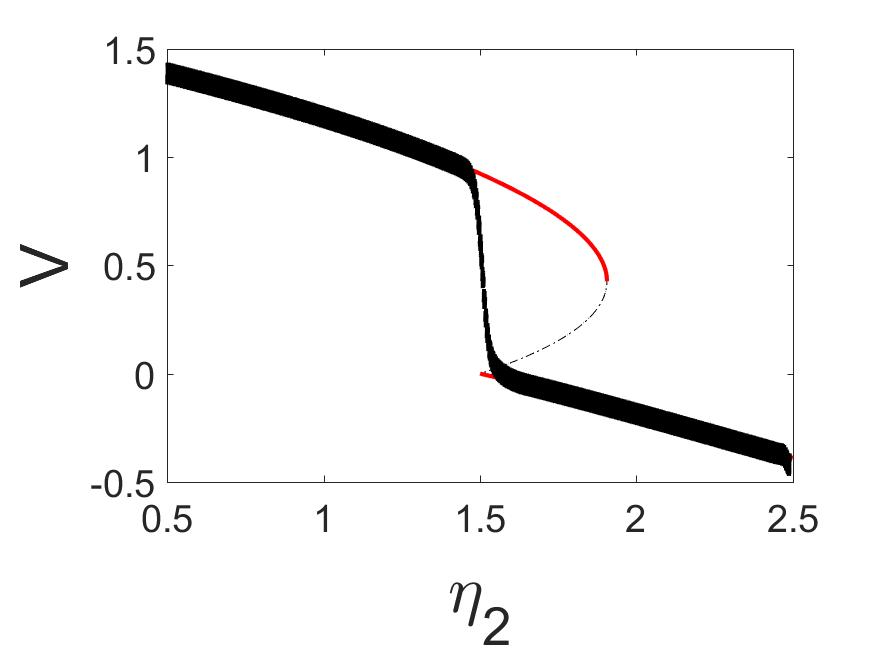
\includegraphics[width=\linewidth]{twoD/slowosc_bif_diagram_small.jpg}
  \caption{}
\end{subfigure}%
\begin{subfigure}{.5\textwidth}
  \centering
  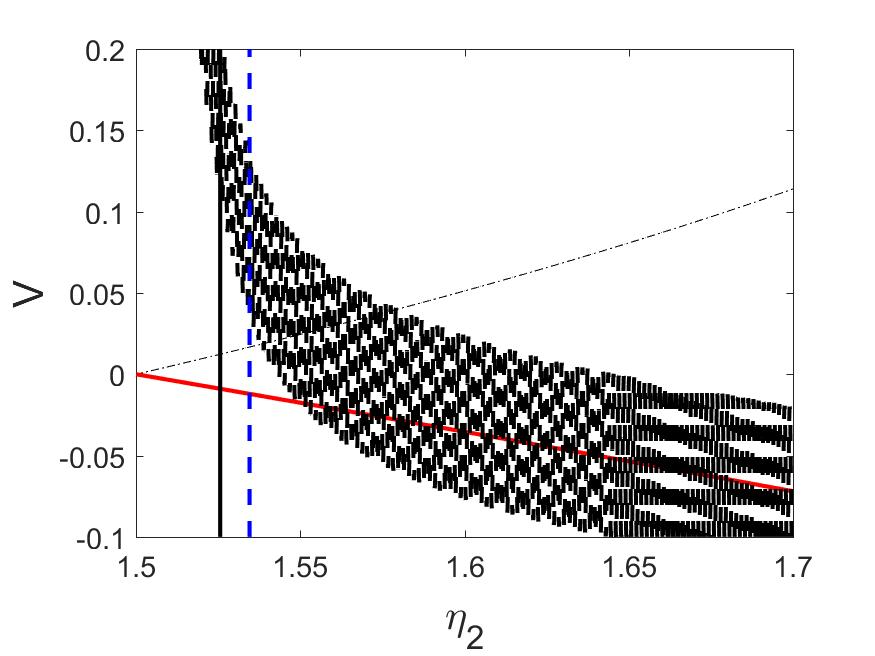
\includegraphics[width=\linewidth]{twoD/slowosc_bif_diagram_small_zoom.jpg}
  \caption{}
\end{subfigure}
\caption{Model values are $\lambda=.8$, $\epsilon=.01$ with $A=B=2$. In (a) the numerical solution (black dotted line) to \eqref{eq:twoD_canonical} is given with $\eta_1=4$, $\eta_3=.375$. In (b) a zoom in closer to the non-smooth bifurcation region where the blue vertical line is the tipping prediction against the black dotted vertical line which is the numerical bifurcation.}
\label{fig:twoD_slowosc_Vnumerics_small}
\end{figure}

\begin{figure}[H]
\centering
\begin{subfigure}{.5\textwidth}
  \centering
  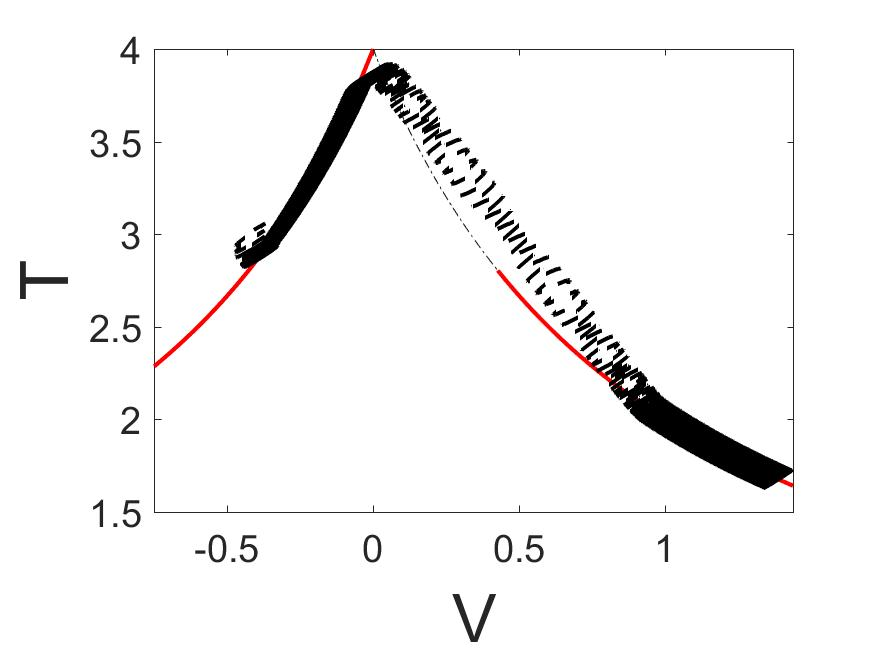
\includegraphics[width=\linewidth]{twoD/slowosc_Tplot_small.jpg}
  \caption{}
\end{subfigure}%
\begin{subfigure}{.5\textwidth}
  \centering
  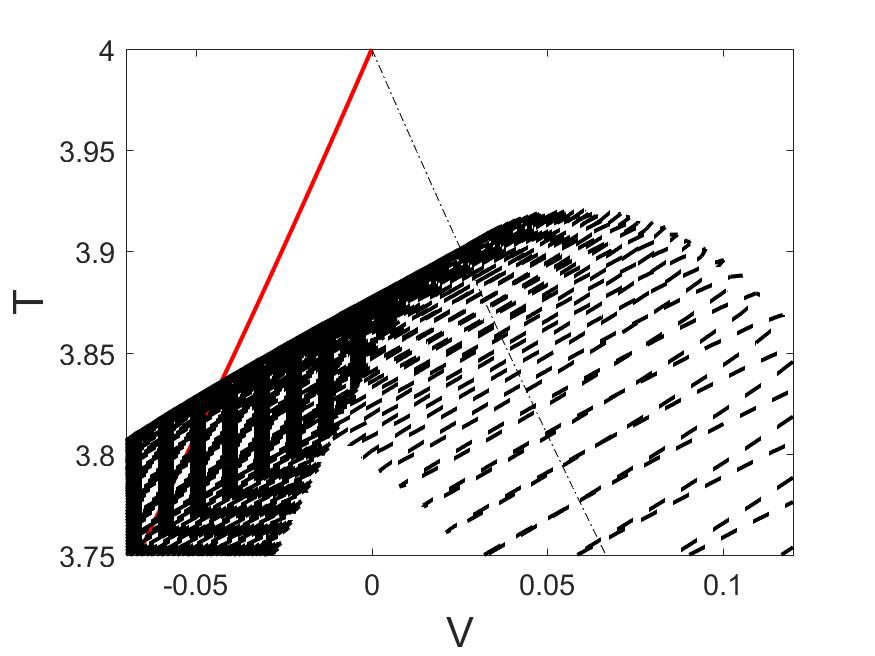
\includegraphics[width=\linewidth]{twoD/slowosc_Tplot_small_zoom.jpg}
  \caption{}
\end{subfigure}
\caption{Model values are $\lambda=.8$, $\epsilon=.01$ with $A=B=2$. In (a) we have the numerical solution (black dotted) over the standard equilibrium plot for $V$ vs. $T$. In (b) a zoom of the bifurcation area.}
\label{fig:twoD_slowosc_Tnumerics_small}
\end{figure}

In figure~\ref{fig:twoD_slowosc_Vnumerics_medium} we have chosen a value of $\lambda$ that causes the tipping to fall into Case II as $\lambda>1$ but this choice is close to the boundary and thus we see comparable behavior to Case I with the addition that the slow variation is now dominant as in \autoref{sec:twoD_slow}. Upon a zoom in, it is apparent that oscillations are still present and this is where we see the mixture of effects that cause a similar tipping to take place. We've plotted the purely slow tipping as the green vertical dotted line for comparison. As the tipping occurs near the purely slow tipping this confirms that the slow variation is indeed dominating the tipping. In figure~\ref{fig:twoD_slowosc_Tnumerics_medium} we again see very similar behavior to the purely slow model in \autoref{sec:twoD_slow} but the zoom in further reveals the oscillations are present and have minor influence by forcing the solution to cross the unstable branch near the tipping.

\begin{figure}[H]
\centering
\begin{subfigure}{.5\textwidth}
  \centering
  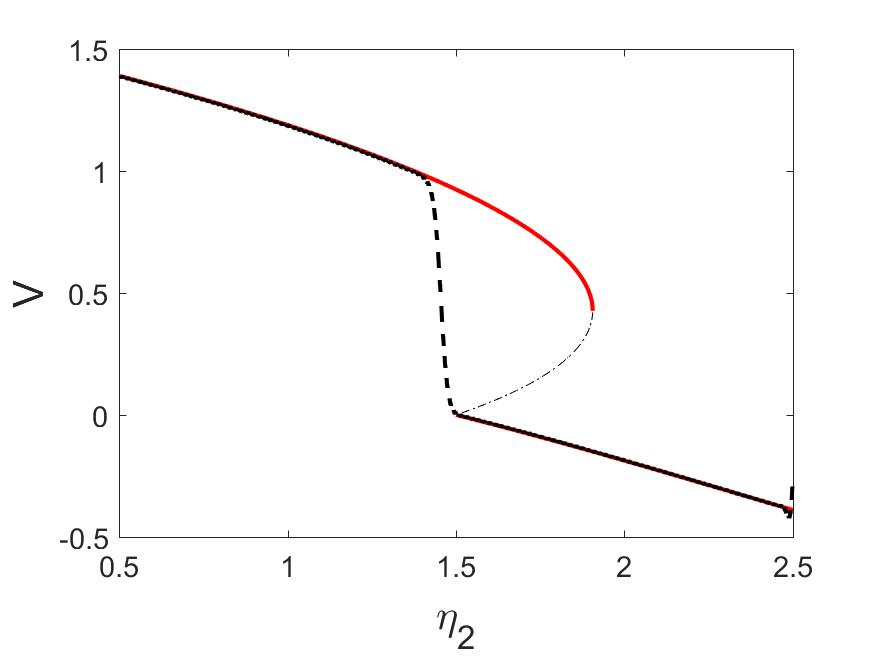
\includegraphics[width=\linewidth]{twoD/slowosc_bif_diagram_medium.jpg}
  \caption{}
\end{subfigure}%
\begin{subfigure}{.5\textwidth}
  \centering
  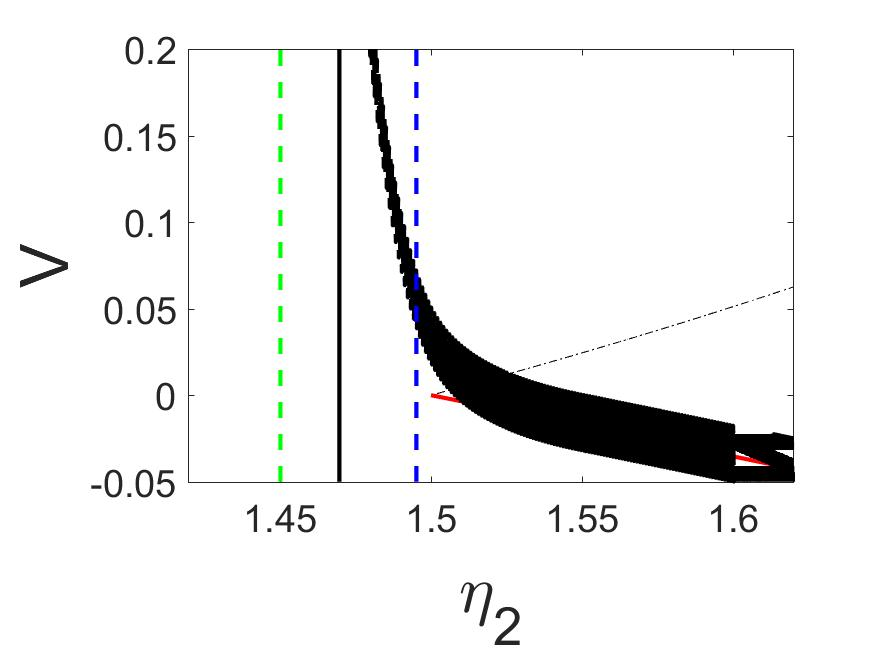
\includegraphics[width=\linewidth]{twoD/slowosc_bif_diagram_medium_zoom.jpg}
  \caption{}
\end{subfigure}
\caption{Model values are $\lambda=1.3$, $\epsilon=.01$ with $A=B=2$. In (a) the numerical solution (black dotted line) to \eqref{eq:twoD_canonical} is given with $\eta_1=4$ and $\eta_3=.375$. In (b) a zoom in closer to the non-smooth bifurcation region where the blue dotted vertical line is the prediction against the black solid vertical line which is the numerical bifurcation.}
\label{fig:twoD_slowosc_Vnumerics_medium}
\end{figure}

\begin{figure}[H]
\centering
\begin{subfigure}{.5\textwidth}
  \centering
  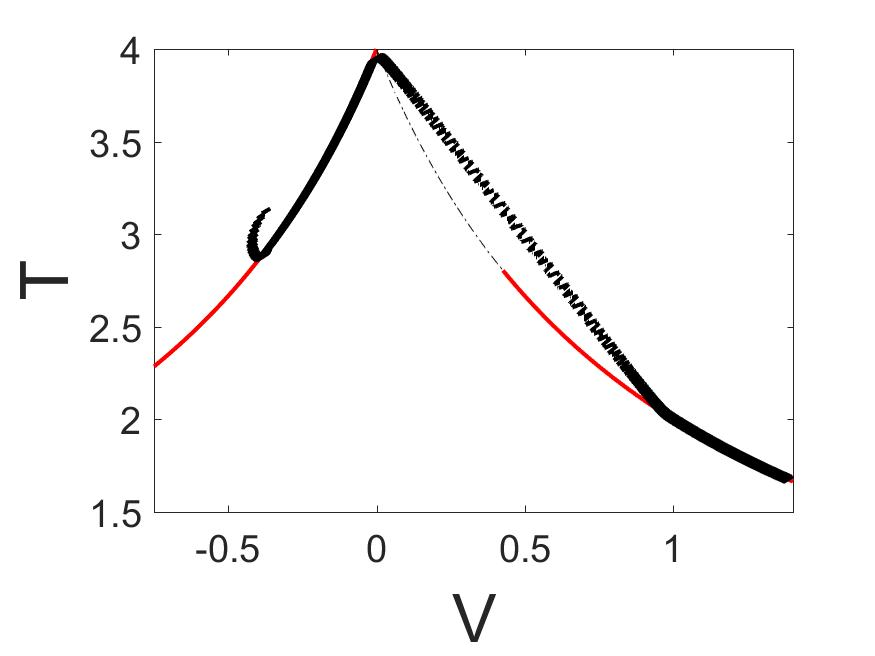
\includegraphics[width=\linewidth]{twoD/slowosc_Tplot_medium.jpg}
  \caption{}
\end{subfigure}%
\begin{subfigure}{.5\textwidth}
  \centering
  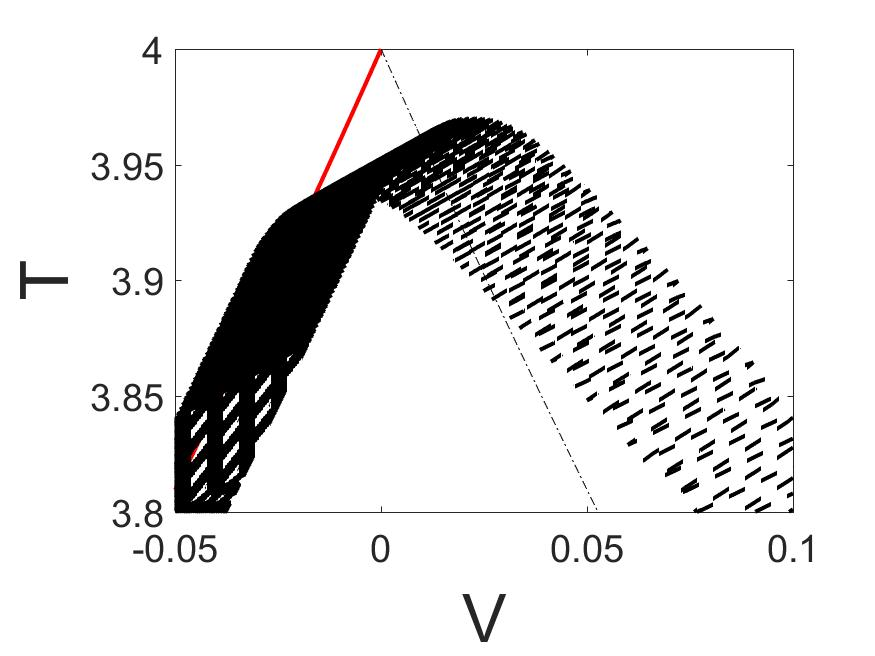
\includegraphics[width=\linewidth]{twoD/slowosc_Tplot_medium_zoom.jpg}
  \caption{}
\end{subfigure}
\caption{Model values are $\lambda=1.3$, $\epsilon=.01$ with $A=B=2$. In (a) we have the numerical solution (black dotted) over the standard equilibrium plot for $V$ vs. $T$. In (b) a zoom of the bifurcation area.}
\label{fig:twoD_slowosc_Tnumerics_medium}
\end{figure}

In figure~\ref{fig:twoD_slowosc_Vnumerics_large} we see the numerics for a $\lambda$ that is large enough to force the problem to behave like the purely slow model like in \autoref{sec:twoD_slow}. Even upon a zoom it is almost impossible to notice that oscillations are occurring in this solution. The green dotted vertical line is our purely slow tipping estimate \eqref{eq:twoD_slow_tipping} where the blue dotted is the same mixed approximation \eqref{eq:twoD_slowosc_subcaseII_tipping}. Further evidence is seen in figure~\ref{fig:twoD_slowosc_Tnumerics_large} where this compares very similar to \eqref{fig:twoD_slow_Tnumerics}.

\begin{figure}[H]
\centering
\begin{subfigure}{.5\textwidth}
  \centering
  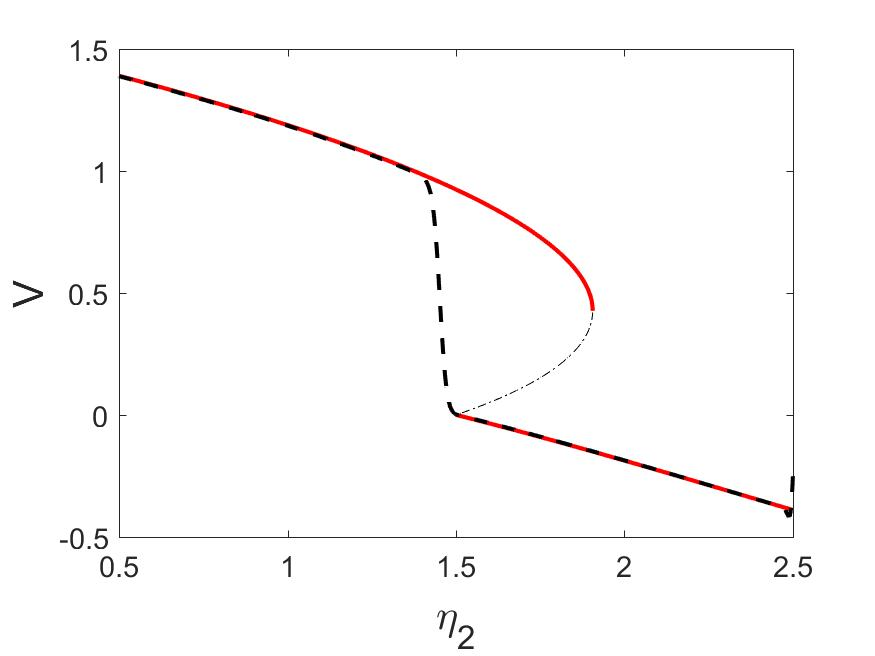
\includegraphics[width=\linewidth]{twoD/slowosc_bif_diagram_large.jpg}
  \caption{}
\end{subfigure}%
\begin{subfigure}{.5\textwidth}
  \centering
  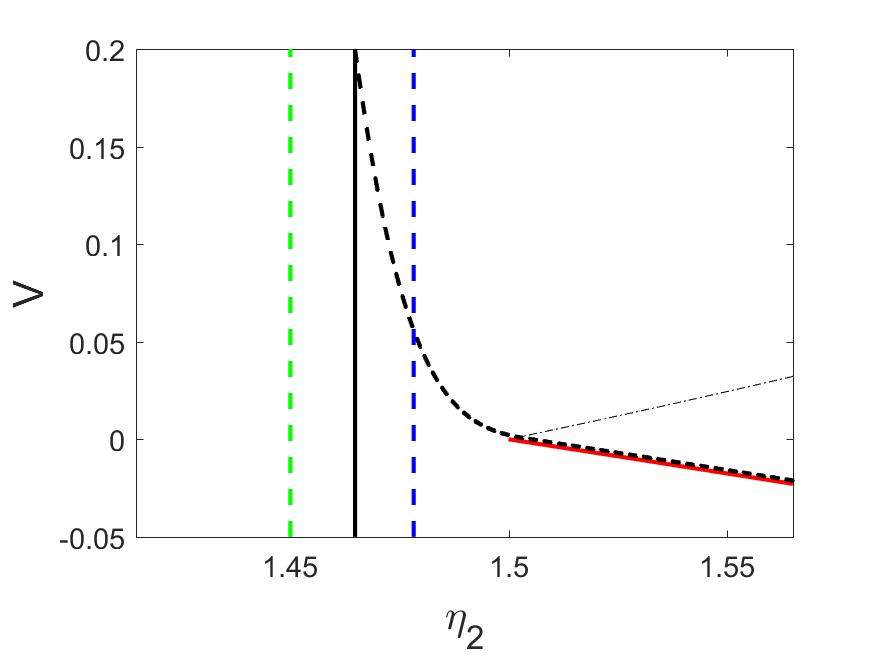
\includegraphics[width=\linewidth]{twoD/slowosc_bif_diagram_large_zoom.jpg}
  \caption{}
\end{subfigure}
\caption{ Model values are $\lambda=2$, $\epsilon=.01$ with $A=B=2$. In (a) the numerical solution (black dotted line) to \eqref{eq:twoD_canonical} is given with $\eta_1=4$ and $\eta_3=.375$. In (b) a zoom in closer to the non-smooth bifurcation region where the blue vertical line is the prediction against the black dotted vertical line which is the numerical bifurcation.}
\label{fig:twoD_slowosc_Vnumerics_large}
\end{figure}

\begin{figure}[H]
\centering
\begin{subfigure}{.5\textwidth}
  \centering
  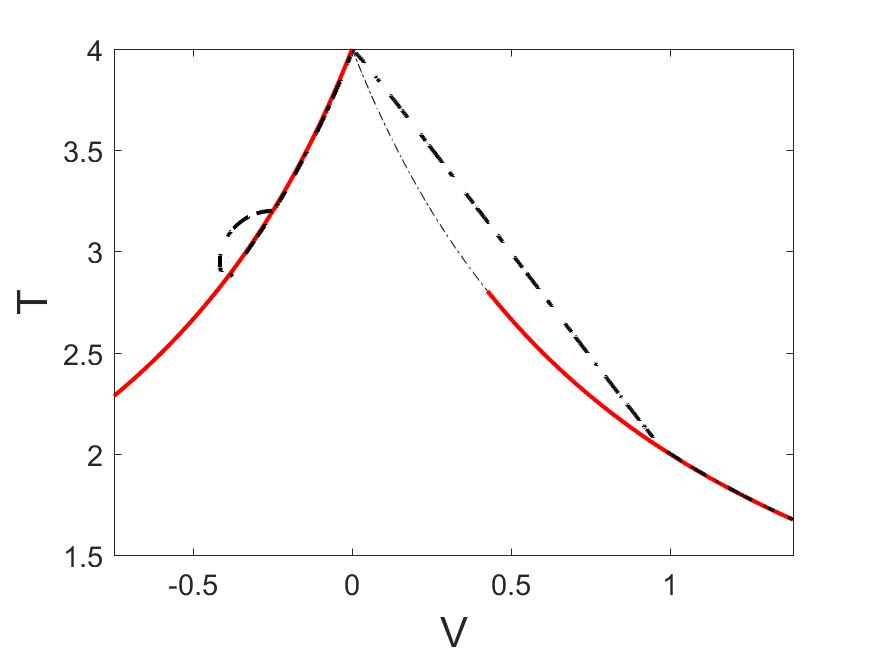
\includegraphics[width=\linewidth]{twoD/slowosc_Tplot_large.jpg}
  \caption{}
\end{subfigure}%
\begin{subfigure}{.5\textwidth}
  \centering
  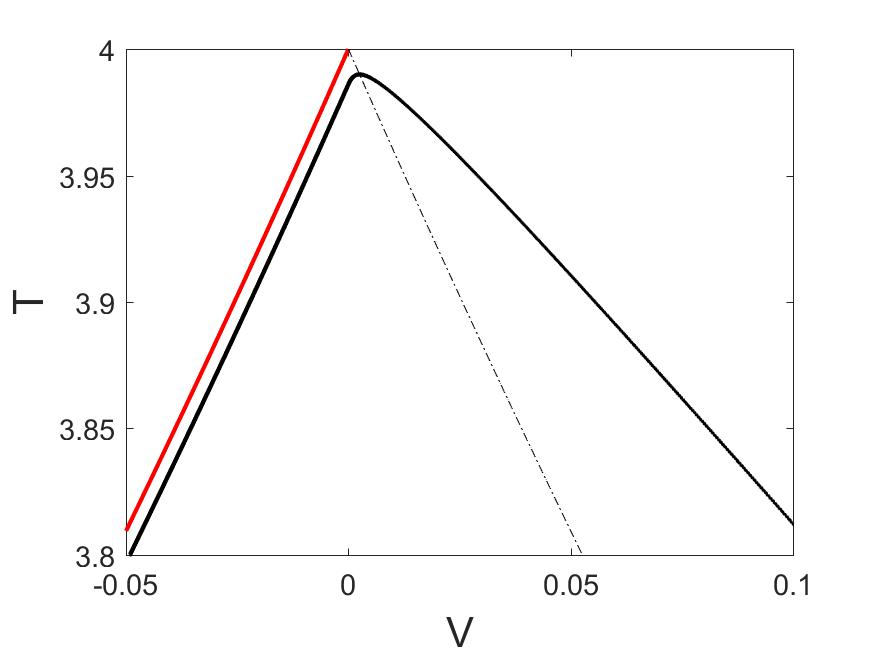
\includegraphics[width=\linewidth]{twoD/slowosc_Tplot_large_zoom.jpg}
  \caption{}
\end{subfigure}
\caption{Model values are $\lambda=2$, $\epsilon=.01$ with $A=B=2$. In (a) we have the numerical solution (black dotted) over the standard equilibrium plot for $V$ vs. $T$. In (b) a zoom of the bifurcation area.}
\label{fig:twoD_slowosc_Tnumerics_large}
\end{figure}

Although the figures above show that we have classified the behavior appropriately for the various cases in $\lambda$ and relative solution sized, performance of our approximate tipping needs to be evaluated to verify our analysis had good results. In figure~\ref{fig:twoD_slowosc_lambdacomp} we compare the tipping between Case I and Case II with the numerical tipping across $\lambda$ with a fixed $\epsilon$. For smaller $\lambda$, the frequency $\Omega$ gets smaller and the Case I tipping becomes more predominant. But for the analysis performed in this section, $\Omega\gg 1$ and for $\lambda<\frac{1}{2}$ we have $\Omega\sim O(1)$. We will not consider low frequency corresponding to $\lambda<\frac{1}{2}$ in this section. The larger $\lambda$ becomes, the less effect we see from the oscillatory forcing until it is negligible for some $\lambda>1$. We notice that our one-dimensional reduction tipping approximation, there is some bias due to this being a reduced approach, there is likely a slightly bigger coefficient and this becomes apparent for $\lambda>1$. Although we use a one-dimensional reduced equation to get these approximations, they seem to be performing quite well across all $\lambda$ hence validating the method developed for tipping with varying $\lambda$.

\begin{figure}[H]
\centering
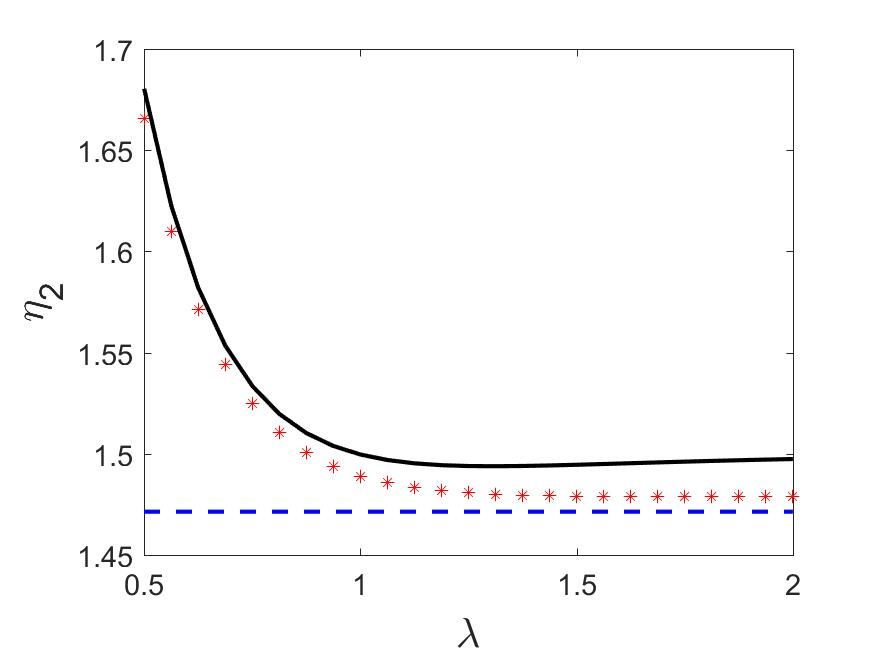
\includegraphics[width=0.7\textwidth]{twoD/slowosc_lambdacomp.jpg}
\caption{An example of numerical tipping (red stars) as the numerical solution to \eqref{eq:oneD_canonical} passes $x=.2$ for the last time. Parameter values are $\epsilon=.01$ and $A=1$. The lines are the Case I tipping estimate (black solid line) and the Case II tipping estimate (blue dotted line).}
\label{fig:twoD_slowosc_lambdacomp}
\end{figure} 

We also are interested in the performance of the tipping approximations across values of $\epsilon$ while leaving $\lambda$ fixed. The performance of each estimate is seen in figure~\ref{fig:twoD_slowosc_epscomp}. For Case I tipping, the range of appropriate $\epsilon$ is highly dependent on the choice in $\lambda$. Often, the range is very small to get accurate estimates. Once this range is left, there are interesting phase effects for the tipping which causes oscillations in the numeric tipping points. For Case II tipping, we that there is a transition happening towards the purely slow tipping, similarly to \autoref{sec:twoD_slow}


\begin{figure}[H]
\centering
\begin{subfigure}{.5\textwidth}
  \centering
  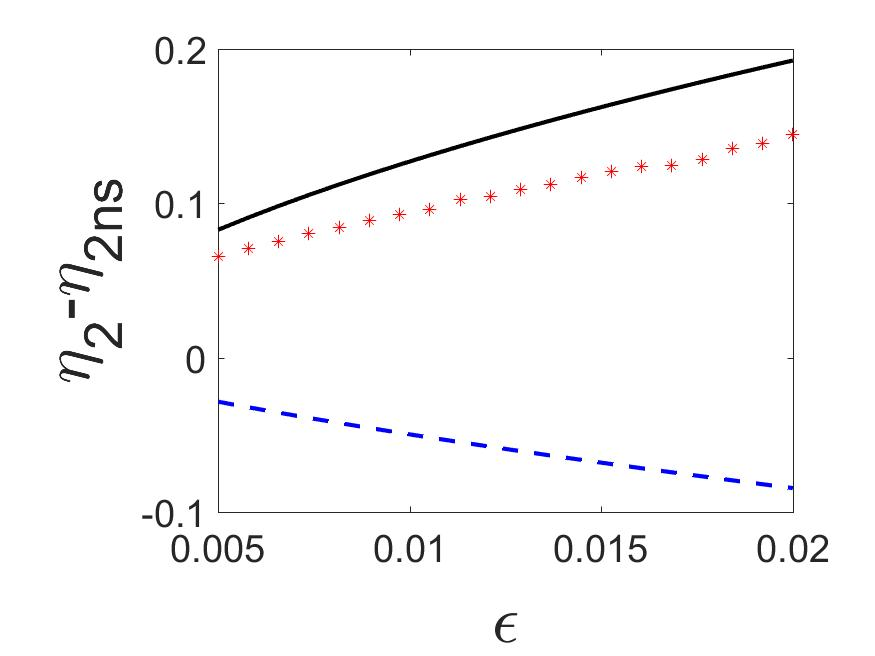
\includegraphics[width=\linewidth]{twoD/slowosc_epscomp_mixed.jpg}
  \caption{$\lambda=.8$}
\end{subfigure}%
\begin{subfigure}{.5\textwidth}
  \centering
  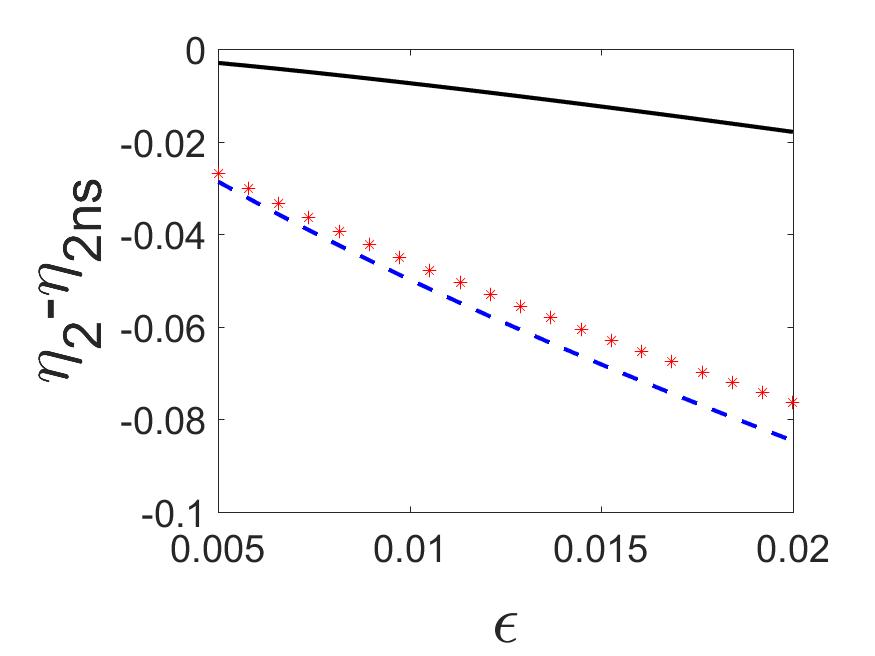
\includegraphics[width=\linewidth]{twoD/slowosc_epscomp_slow.jpg}
  \caption{$\lambda=1.3$}
\end{subfigure}
\caption{The numerical tipping (red stars) follows the appropriate case depending on $\lambda$ for $\epsilon=0.005$. The Case I tipping estimate (black solid line) and purely slow tipping estimate (blue dotted line) are shown.}
\label{fig:twoD_slowosc_epscomp}
\end{figure}

With the numerical results agreeing with our results, we may finally conclude that this method is both useful for analyzing the non-smooth behavior in the Stommel model but also results in an approximation that is more accurate in the extremes of the model (i.e $\Omega \gg 1$ or $\epsilon \ll 1$). This gives us a very accessible means of extracting the tipping in the full two-dimensional without needing to solve difficult Riccati equations or other complex systems that appear from the full problem. All that is needed to verify is our solutions remain stable until we arrive at the region of tipping.

\subsection{Stability}

\subsubsection{Case I: $\lambda\le 1$}

From the analysis, we had discovered the inner equations that govern the behavior of the solution for this range of $\lambda$ are

\begin{equation}\label{eq:twoD_slowosc_stability_caseI_full}
\begin{aligned}
{P_0}_t =& -\epsilon^{1-\lambda} n(t)-\eta_2 P_0 -(1-\eta_3)Q_0,\\
{Q_0}_t =& -\frac{\eta_1}{2\pi}\int_0^{2\pi}|P_0-A\cos(R)|\,dR - Q_0.
\end{aligned}
\end{equation}

But we also found that the relative size of $P_0(t)$ dictates the difficulty of \eqref{eq:twoD_slowosc_stability_caseI_full}. In the analysis we treat these as Sub-Case I: $P_0(t)\le-|A|$ and Sub-Case II: $|P_0(t)|<|A|$ which each require a separate analysis due to their differing behavior.

\subsubsection{Sub-Case I: $P_0(t)\le-|A|$}

We called this the entirely below-axis sub-case due to the solution remaining below the axis and hence predictable under these conditions thus we anticipate this sub-case to remain stable. The equation \eqref{eq:twoD_slowosc_stability_caseI_full} simplifies for this sub-case to

\begin{equation}\label{eq:twoD_slowosc_stability_subcaseI_full}
\begin{aligned}
{P_0}_t =& -\epsilon^{1-\lambda} n(t)-\eta_2 P_0 -(1-\eta_3)Q_0,\\
{Q_0}_t =& \eta_1 P_0 - Q_0.
\end{aligned}
\end{equation}

Which from the analysis we choose to reduce \eqref{eq:twoD_slowosc_stability_subcaseI_full} with the pseudo-equilibria $Q_0(P_0)=\eta_1 P_0$. This gives the following one-dimensional equation with it's pseudo-equilibria as 

\begin{equation}\label{eq:twoD_slowosc_stability_subcaseI_reduced}
\begin{aligned}
{P_0}_t =& -\epsilon^{1-\lambda}n(t)-(\eta_3+\eta_1(1-\eta_3))P_0=f(t,P_0),\\ Z^0(t) =& -\epsilon^{1-\lambda}\frac{n(t)}{\eta_3+\eta_1(1-\eta_3)}.
\end{aligned}
\end{equation}

We adopt a similar strategy for analyzing the stability from the one-dimensional model in \autoref{sec:oneD_slowosc} due to \eqref{eq:twoD_slowosc_stability_subcaseI_reduced} being a one-dimensional equation. Hence we take a simple linear perturbation about the pseudo-equilibrium with $P_0(t)=Z^0(t)+U(t)$ and $\lVert U(t)\rVert \ll 1$. Taking special care to note that $Z^0(t)$ also varies in time, we find the Taylor approximation

\begin{equation}\label{eq:twoD_slowosc_subcaseI_perturb}
\begin{aligned}
{P_0}_t=&f(t,Z^0) +f_{P_0}(t,Z^0)(P_0(t)-Z^0(t))+O(\lVert (P_0(t)-Z^0(t))^2\rVert^2),\\
U_t+Z^0_t =& -(\eta_3+\eta_1(1-\eta_3))U,\\
U_t =& -\epsilon^{1-\lambda}\frac{1}{\eta_3+\eta_1(1-\eta_3)}-(\eta_3+\eta_1(1-\eta_3))U.
\end{aligned}
\end{equation}

With \eqref{eq:twoD_slowosc_subcaseI_perturb} we find that the perturbations decay exponentially to a nearby equilibrium. This indicates the solution for this sub-case is hyperbolically stable and further agrees that no tipping will happen for this size of the solution.

\subsubsection{Sub-Case II: $|P_0(t)|<-|A|$}

We called this the crossing case and from the analysis we anticipate the tipping to occur as the solution is gradually becoming uncontrollable with the crossing. Under the conditions of this sub-case, we integrate \eqref{eq:twoD_slowosc_stability_caseI_full} with the $R_1$ and $R_2$ from the analysis and take the same Taylor approximation to find 

\begin{equation}\label{eq:twoD_slowosc_stability_subcaseII,full}
\begin{aligned}
{P_0}_t =& -n(t)-\eta_3 P_0-(1-\eta_3)Q_0,\\
{Q_0}_t =&-\epsilon^{\lambda-1}\frac{2\eta_1|A|}{\pi}-\epsilon^{1-\lambda}\frac{\eta_1(1-\eta_3)}{\pi|A|}P_0^2-Q_0.
\end{aligned}
\end{equation}

Once more, we assume that the equation for $Q_0$ is in pseudo-equilibrium 
to reduce to the following one-dimensional inner equation with equilibrium where here we let $a=\frac{\eta_1(1-\eta_3)}{\pi|A|}$ for simplicity

\begin{equation}\label{eq:twoD_slowosc_stability_subcaseII,reduced}
\begin{aligned}
{P_0}_t =& -\epsilon^{1-\lambda}n(t)+\frac{2\eta_1(1-\eta_3)|A|}{\pi}-\eta_3 P_0+aP_0^2=f(t,P_0),\\
Z^0(t) =& \frac{1}{2a}\left(\eta_3-\sqrt{4a(\epsilon^{1-\lambda}n(t)-n_{\text{osc}})}\right).
\end{aligned}
\end{equation}

Where we choose to write the argument of the square root in terms of the bifurcation found in \eqref{eq:twoD_osc_bifurcation}. We then consider the linear perturbation about the pseudo-equilibrium $P_0(t)= Z^0(t)+U(t)$ with $\lVert U\rVert \ll 1$. We take a Taylor expansion here to find the dynamics of the perturbation, but recall that we have contributions to the derivative from both the perturbation as well as the pseudo-equilibrium. This is seen with

\begin{equation}
\begin{aligned}
{P_0}_t =& Z^0_t+U_t,\\
Z^0_t=&\begin{cases}
\frac{\epsilon^{1-\lambda}}{\sqrt{4a(\epsilon^{1-\lambda}n(t)-n_{\text{osc}})}} & \epsilon^{1-\lambda}n(t)>n_{\text{osc}},\\
0 & \epsilon^{1-\lambda}n(t)=n_{\text{osc}}.
\end{cases}
\end{aligned}
\end{equation}

Thus we find the following Taylor expansion for the perturbations

\begin{equation}\label{eq:twoD_slowosc_stability_subcaseII_perturb}
\begin{aligned}
{P_0}_t =& f(t,Z^0)+f_{P_0}(t,Z^0)(P_0-Z^0)+O(\lVert P_0-Z^0 \rVert^2),\\
U_t+Z^0_t=& -\sqrt{4a(\epsilon^{1-\lambda}n(t)-n_{\text{osc}})} U,\\
 U_t = & \begin{cases}
\frac{\epsilon^{1-\lambda}}{\sqrt{4a(\epsilon^{1-\lambda}n(t)-n_{\text{osc}})}}-\left(\sqrt{4a(\epsilon^{1-\lambda}n(t)-n_{\text{osc}})}\right) U & \epsilon^{1-\lambda}n(t)>n_{\text{osc}},\\
0 & \epsilon^{1-\lambda}n(t)=n_{\text{osc}}.
\end{cases}
\end{aligned}
\end{equation}

From \eqref{eq:twoD_slowosc_stability_subcaseII_perturb} we find exponentially decaying perturbations that give asymptotic stability until we get to the oscillatory bifurcation. The oscillatory bifurcation corresponds to non-hyperbolic behavior and we lose stability shortly after which indicates of the tipping to occur after the bifurcation.

\subsubsection{Case II: $\lambda>1$}

From the analysis we determined this to be the slowly dominant case and we had discovered the inner equations that govern the behavior of the solution for this range of $\lambda$ to be

\begin{equation}\label{eq:twoD_slowosc_caseII_full}
\begin{aligned}
{P_0}_t =& - n(t)-\eta_2 P_0 -(1-\eta_3)Q_0,\\
{Q_0}_t =& -\frac{\eta_1}{2\pi}\int_0^{2\pi}|P_0-\epsilon^{\lambda-1} A\cos(R)|\,dR - Q_0.
\end{aligned}
\end{equation}

The behavior of this case when $\lambda\sim 1$ is very similar to Case I, thus we anticipate the stability to behave similarly as well. Hence we consider the behavior when $|P_0(t)|<\epsilon^{\lambda-1}|A|$ which is where we found tipping to occur in the analysis. As long as we have $\epsilon^{\lambda-1}A\sim O(1)$, we are follow the same approach as Case I where we integrate \eqref{eq:twoD_slowosc_caseII_full} with a similar $R_1$ and $R_2$ and use a Taylor approximation to get

\begin{equation*}
\begin{aligned}
{P_0}_t =& - n(t)-\eta_2 P_0 -(1-\eta_3)Q_0,\\
{Q_0}_t =& -\epsilon^{\lambda-1}\frac{2\eta_1(1-\eta_3)|A|}{\pi}-\epsilon^{1-\lambda}\frac{\eta_1}{\pi|A|}P_0^2- Q_0.
\end{aligned}
\end{equation*}

The analysis gave sufficient reason to reduce the inner equations to a one-dimensional model and thus like in Case I w find the inner equation with pseudo-equilibrium where here we let $a=\frac{\eta_1(1-\eta_3)}{\pi|A|}$ for simplicity

\begin{equation*}
\begin{aligned}
{P_0}_t =& -n(t)+\epsilon^{\lambda-1}\frac{2\eta_1(1-\eta_3)|A|}{\pi}-\eta_3 P_0+\epsilon^{1-\lambda}aP_0^2,\\
Z^0(t) =& \frac{1}{2a}\left(\epsilon^{\lambda-1}\eta_3-\sqrt{\epsilon^{\lambda-1}4a(n(t)-\epsilon^{\lambda-1}n_{\text{osc}})}\right)
\end{aligned}
\end{equation*}

Where we consider the linear perturbation about the pseudo-equilibrium $P_0(t)= Z^0(t)_U(t)$ with $\lVert U\rVert \ll 1$. We take a Taylor expansion here to find the dynamics of the perturbation, but recall that we have contributions to the derivative from both the perturbation as well as the pseudo-equilibrium. This is seen with

\begin{equation}
\begin{aligned}
{P_0}_t =& Z^0_t+U_t,\\
Z^0_t=&\begin{cases}
\frac{\epsilon^{(\lambda-1)/2}}{\sqrt{4a(n(t)-\epsilon^{\lambda-1}n_{\text{osc}})}} & n(t)>\epsilon^{\lambda-1}n_{\text{osc}},\\
0 & n(t)=\epsilon^{\lambda-1}n_{\text{osc}}.
\end{cases}
\end{aligned}
\end{equation}

Thus we find the following Taylor expansion for the perturbations

\begin{equation}\label{eq:twoD_slowosc_stability_caseII_perturb}
\begin{aligned}
{P_0}_t =& f(t,Z^0)+f_{P_0}(t,Z^0)(P_0-Z^0)+O(\lVert P_0-Z^0 \rVert^2),\\
U_t+Z^0_t=& -\left(\sqrt{\epsilon^{1-\lambda}4a(n(t)-\epsilon^{\lambda-1}n_{\text{osc}})}\right) U,\\
U_t = & \begin{cases}
\frac{\epsilon^{(\lambda-1)/2}}{\sqrt{4a(n(t)-\epsilon^{\lambda-1}n_{\text{osc}})}}-\left(\sqrt{\epsilon^{1-\lambda}4a(n(t)-n_{\text{osc}})}\right) U & n(t)>\epsilon^{\lambda-1}n_{\text{osc}},\\
0 & n(t)=\epsilon^{\lambda-1}n_{\text{osc}}.
\end{cases}
\end{aligned}
\end{equation}

From \eqref{eq:twoD_slowosc_stability_caseII_perturb} we find that the perturbations decay exponentially and we have asymptotic stability until we get to the oscillatory bifurcation. The bifurcation found in \eqref{eq:twoD_osc_bifurcation} corresponds to non-hyperbolic behavior and we then lose the stability which indicates of the tipping to occur after the bifurcation. Comparing this to Case I, we see there is small nuances between these perturbations, although the overall stability remains the same. As for when $\lambda$ grows, we already established this behaves like the purely slow model and hence we can use the stability from that section to conclude that our solution is still stable until the slow tipping point, at which we lose stability as anticipated.


Thus the stability for both Case I and Case II agrees with the results found in the analysis. We have that the behavior of the solution is stable from the outer solution, stability holds before the solution begins to cross the axis $V=0$ and once the crossing begins to happen we lose stability at the location of the oscillatory bifurcation. Because there is slow variation in this model, there is still delayed behavior and thus the tipping happens shorty after the oscillatory bifurcation. In both cases we discovered that the pseudo-equilibrium has a contribution to the derivative and this in turn causes the perturbations to decay towards a small constant. This means that there is a small region around the pseudo-equilibrium that attracts the solution and this is seen in the numerical results. 
